\documentclass[a4paper,12pt]{article}

% Pakete laden
\usepackage[T1]{fontenc}
\usepackage[utf8]{inputenc}
\usepackage[ngerman]{babel}
%\usepackage{lmodern}
\usepackage{geometry}
%\usepackage{setspace}
\usepackage{graphicx}
%\usepackage{amsmath}
%\usepackage{amssymb}
%\usepackage{booktabs}
%\usepackage{natbib}
%\usepackage{tikz}
%\usepackage{caption}
%\usepackage{listings}
%\usepackage{ragged2e}
%\usetikzlibrary{positioning}
%\usetikzlibrary{shapes}
%\usepackage{afterpage}
%\usepackage{float}
%\usepackage{titlesec}
\usepackage{hyperref}%hyperref links

\usepackage{fancyhdr}%footer
\usepackage{graphicx}%images
\usepackage{wrapfig}%images in text
\usepackage{adjustbox}
\usepackage{pdfpages}  % Include this line to use the pdfpages package
\usepackage{longtable}%for table that spread over multiple pages
\usepackage{float}%fix figure position
%\usepackage{lastpage}
\usepackage[yyyymmdd]{datetime}%display the date better
\renewcommand{\dateseparator}{-}

%\bibliographystyle{unsrt}





% Kopfzeile
\pagestyle{fancy}
\fancyhf{}
\fancyhead[L]{\includegraphics[width=5 cm]{OST_Logo.png}}
\fancyhead[R]{Maschinentechnik | Innovation}
\geometry{headsep=1.6cm}%sonst fängt das logo zu weit unten

% Fusszeile 
\rfoot{Seite \thepage}
%\rfoot{\thepage}
\renewcommand{\footrulewidth}{0pt}
\fancyfoot[L]{Peter Kuhn} % author on the left
\fancyfoot[C]{Semesterarbeit HS 2023} % title in the c enter




% Titelblatt
\begin{document}


\begin{titlepage}
  \end{titlepage}
% Import the PDF
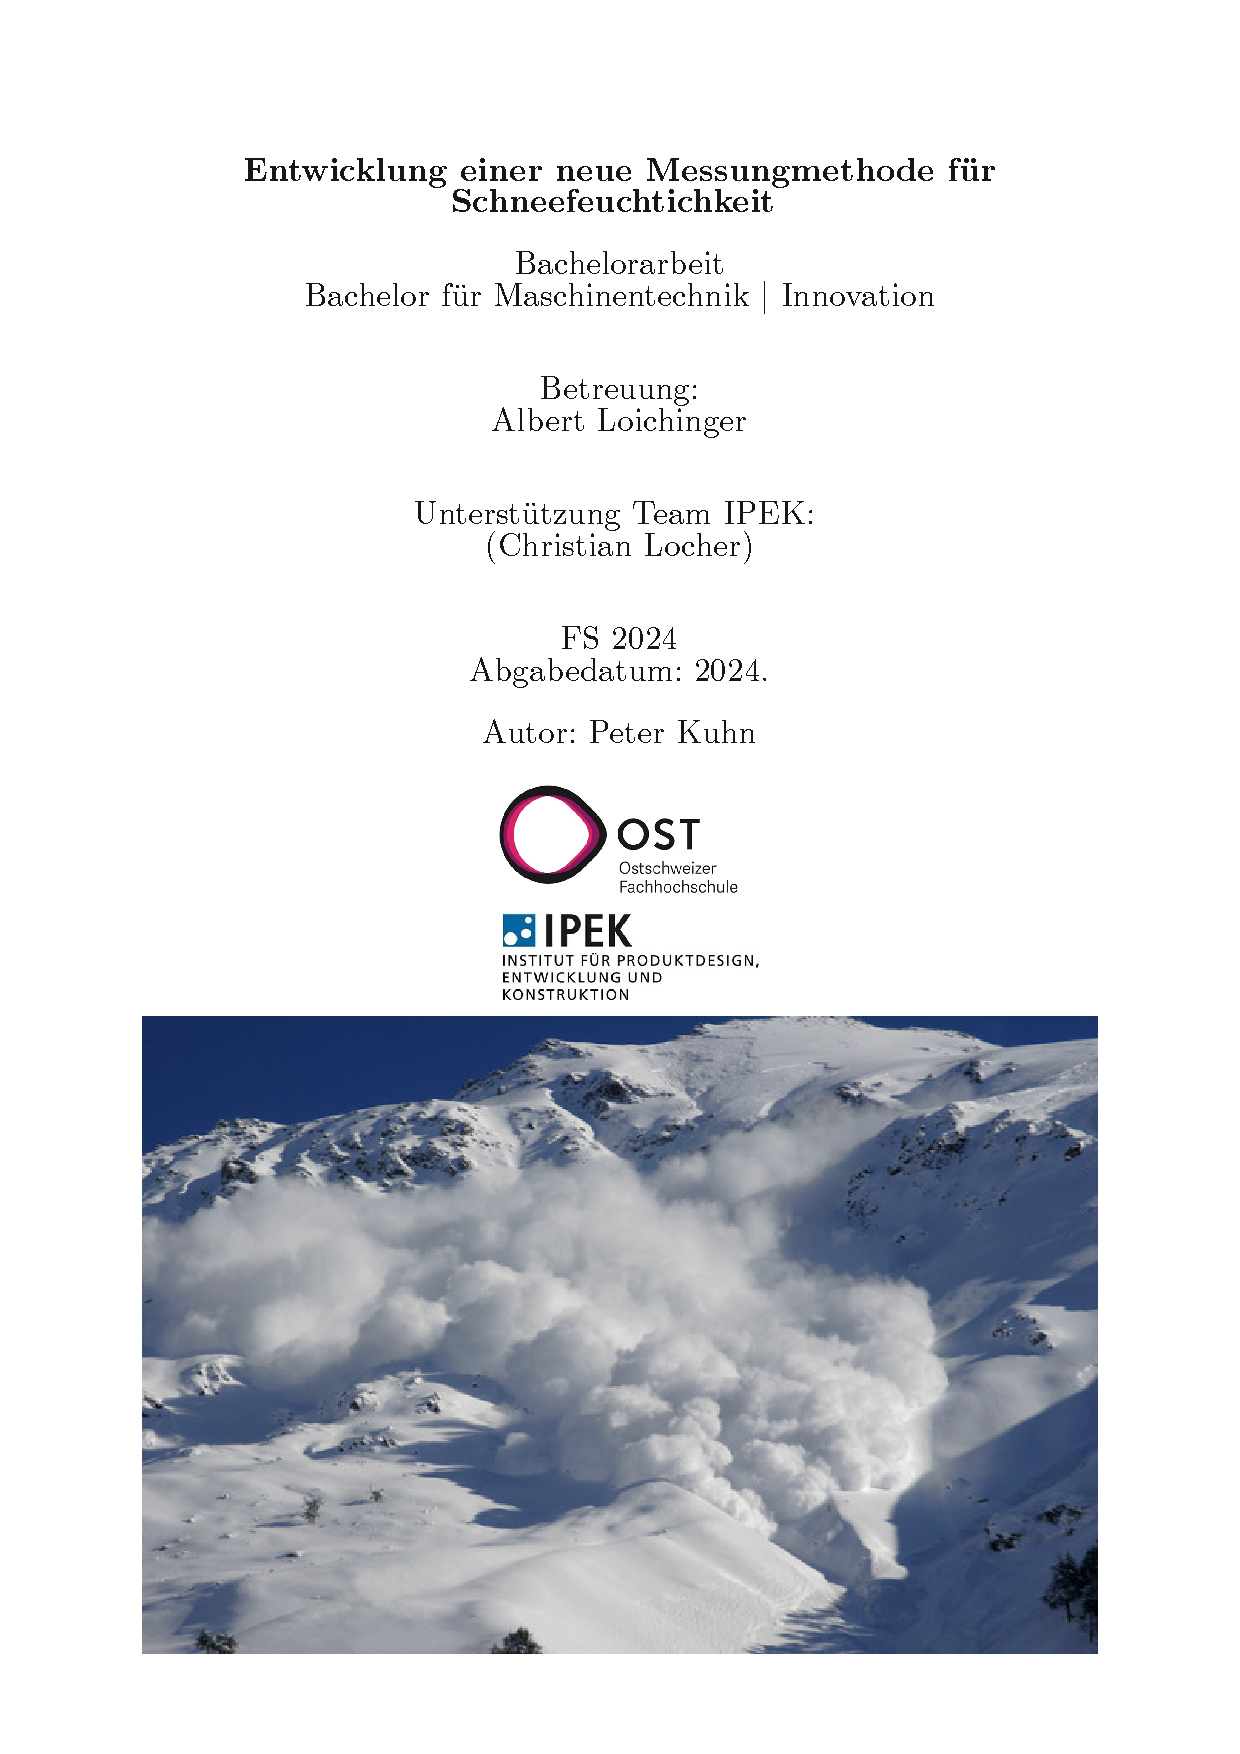
\includepdf{Titelseite.pdf}
%import something from scribus


\pagestyle{empty}
\section*{Abstract}


\iffalse

Dazu habe ich unterschiedliche  physikalische Wirkprinzipien getestet. 
Die vielversprechendste Technik basiert auf einem Water Indikator Tape- das ursprünglich für die Elektronik entwickelt wurde und  das visuell ausgewertet wird.

 Für eine definierte Zeitspanne wird das Tape auf die Schneeoberfläche gelegt. Anschliessend wird es fotografiert. Die Auswertung erfolgt durch visuelle und digitale Analyse.
Das Produkt durchlief 5 Iterationen. Die entwickelte Messtechnik zeigt die Fähigkeit, die Interaktion des gefrorenen und des flüssigen Wassers mit dem Tape zu erfasseberfasst werden.

Weitere Optimierung und Testung ist erforderlich, um die Genauigkeit und Präzision des Sensors zu gewährleisten.

Dies ist Voraussetzung dafür, den Sensor in der Zukunft zu einem marktfähigen Produkt weiter entwicklen zu können.

Die Ergebnisse dieser Arbeit können einen Beitrag zur Weiterentwicklung von Messmethoden für den LWC im Schnee leisten. Eine  verbesserte Vorhersage von Gleitschneelawinen ermöglicht adäquate Reaktionen auf dieses Naturereignis. 




in dieser produktentwicklungsaufgabe wurde eine Innovativer sensor entwickelt um den Liquid water Contet von schnee zu messen.

dazu wurden verschiedene physikalische wirkprinzipien getesten. die vielversprechendste technik in der ein Water indikator Tape aus der qualitassicherung im elektronikbrachnche visuell auswertet wird, wurde uber 5 iterationen entwickelnt um die interaktion des schnees und Taps zu verstehen.


Die messmethode zeigt die fahigkeiten den lwc von schnee zu erfassen. bis jetzt ist es aber noch nicht sicher ob die prazision und genauigkeit ausreichend ist um in ein produkt umgesetzt zu werden.


In dieser Arbeit wurde ein innovativer Sensor zur Messung des Flüssigwassergehalts (Liquid Water Content, LWC) in Schnee entwickelt. Verschiedene physikalische Prinzipien wurden getestet, um die beste Methode zur Bestimmung des LWC zu identifizieren. Die vielversprechendste Technik erwies sich als der Einsatz eines Wasserindikatorbands aus der Qualitätssicherung in der Elektronikbranche, welches visuell ausgewertet wird. Über fünf Iterationen hinweg wurde der Sensor weiterentwickelt, um die Interaktion zwischen Schnee und dem Indikatorband besser zu verstehen.

Die Auswertung erfolgt durch visuelle und digitale Analyse des 3M 5559 Water Indikator Tapes. Das Tape, das bei Kontakt mit Wasser rot wird, wird für definierte Zeitspannen auf die Schneeoberfläche gelegt und anschließend fotografiert. Die visuelle Beurteilung erfolgt durch die einfache Betrachtung der roten Verfärbung auf dem Tape. Für eine präzisere Analyse wird die Bildverarbeitung eingesetzt, bei der Software den Anteil der roten zu weißen Fläche berechnet, um den Flüssigwassergehalt zu quantifizieren.

Die entwickelte Messtechnik zeigt die Fähigkeit, den LWC im Schnee zu erfassen, jedoch ist die Präzision und Genauigkeit der Messungen noch nicht ausreichend, um den Sensor als marktfähiges Produkt zu etablieren. Weitere Optimierungen und umfangreiche Tests sind erforderlich, um die Zuverlässigkeit und Praktikabilität des Sensors zu gewährleisten. Die Ergebnisse dieser Arbeit liefern einen wichtigen Beitrag zur Weiterentwicklung von Messmethoden für den LWC im Schnee und könnten zukünftig zur Verbesserung der Vorhersage und Prävention von Gleitschneelawinen beitragen.

\fi

\subsection*{Beschreibung der Abkürzungen}
\begin{acronym}[XXXXX]
    \setlength{\itemsep}{-\parsep}
    \acro{BA}{Bachelorarbeit}
    \acro{LWC}{Liquid Water Content}
    \acro{SLF}{Schweizerisches Institut für Schnee- und Lawinenforschung}
    \acro{IPEK}{Institut für Produktentwicklung}
    \acro{TRL}{Technology Readiness Level}
    \acro{ML}{Maschinelles Lernen}
    \acro{IR}{Infra Rot}
    \acro{FDM}{Fused Deposition Modeling}
    \acro{FS}{Fruhlings Semester}
    \acro{OST}{Ost schweizer fachhochschule}
    \acro{MHz}{mega Herz}
    \acro{GPS}{gobal positioning system}
    \acro{Mri}{magnetic resonacn imaging}
    \acro{Tape}{Water indicator tape 5559 von 3M}
    \acro{CAD}{computer aided design}
    \acro{RGB}{Rot Grun blau}
    \acro{DB}{Daten Bank}
    \acro{xps}{extruded polystyrene}
\end{acronym}

% Inhaltsverzeichnis
\tableofcontents
%\pagenumbering{Roman}
\newpage
\pagestyle{fancy}

\setcounter{page}{1}
\section{Einleitung}
Ziel dieser Arbeit ist, einen Sensor zu entwickeln, der flüssiges Wasser im Schnee misst.

Das flüssige Wasser im Schnee ist ein entscheidender Parameter um das Verhalten des Schnees an einem lawinen gefährdeten Hang  vorherzusagen. Seit 40 Jahren wird das Thema erforscht,  und es gibt unterschiedliche Methoden das heterogene Gemisch aus festen, flüssigen und gasförmigen Stoffen, diesen Schaum aus Eis, Wasser und Luft zu messen.

Die vorhandenen Geräte nutzen unterschiedliche Ansätze, haben aber teils  Nachteile zum Beispiel dass sie das Verhältnis von flüssigem Wasser zum Schnee nicht in einem Arbeitsschritt erfassen.

Ich habe verschiedene theoretische Ansätze der Produktentwicklung im Verlauf der Bachelorarbeit genutzt.

Um den Sensor herzustellen habe ich entsprechend der agilen hardware Entwicklung möglichst rasch Iterationen von Sensoren als Produkt hergestellt, getestet und angepasst.

\iffalse
ziel dieser Arbeit ist die entwicklung eines innovativen sensors um die scheefeuchtigkeit zu messen.

Die schneefeuchtigkeit ist ein entscheidenen Parameter um Gleitschneelawinen abzuschetzten. seit 40 jahren ist wird Thema beforscht. Es gibt verschiedenste Techniken um den Schaum aus Eis, Wasser und Luft zu messen. heutige Produkte konnen den LWC messen, haben aber verschiedene schwerwigeende nachteile.

um dieses Produktentwicklung an zu gehen werden verschiedene techniken der Produktentwicklung eingesetzt. um ein sensor zu erreichen der einsatztfahig ist, wurde nach aglier hardware entwicklung moglichst schnell Itterationen von sensoren entwickelt.

\fi


\section{Grundlagen}
\subsection{Herstellungsprozess des Spritzgiessen}
Spritzguss ist ein Fertigungsprozess zur Herstellung von Teilen durch das Einspritzen von geschmolzenem Material in eine Form. Der Spritzguss kann mit einer Vielzahl von Materialien durchgeführt werden, hauptsächlich Metalle (wofür der Prozess als Druckguss bezeichnet wird), Gläser, Elastomere, Süsswaren und am häufigsten thermoplastische und duroplastische Polymere. Material für das Teil wird in ein beheiztes Fass eingespeist, gemischt (unter Verwendung einer Schneckenwelle) und in eine Kavität eingespritzt, wo es abkühlt und sich der Formgebung der Form anpasst. Nachdem ein Produkt entworfen wurde, normalerweise von einem Industriedesigner oder Ingenieur, werden Formen \ref{fig:Werkzeugu} von einem Werkzeugmacher aus Metall hergestellt, normalerweise entweder aus Stahl oder Aluminium, und präzisions gefertigt, um die Merkmale des gewünschten Teils zu bilden. Der Spritzguss wird weitgehend für die Herstellung verschiedener Teile verwendet, von den kleinsten Komponenten bis zu ganzen Karosserieteilen von Autos.



Der Spritzguss verwendet eine spezielle Maschine mit drei Hauptteilen: der Einspritzeinheit, der Form und der Klemme. Teile, die spritzgegossen werden sollen, müssen sehr sorgfältig entworfen werden, um den Spritzgussprozess zu erleichtern. Dabei müssen das für das Teil verwendete Material, die gewünschte Form und Merkmale des Teils, das Material der Form und die Eigenschaften der Spritzgussmaschine alle berücksichtigt werden. Die Vielseitigkeit des Spritzgusses wird durch diese Vielfalt an Design-Überlegungen und Möglichkeiten erleichtert.

\begin{figure}%r and l for right and left
   
  \includegraphics[width=0.48\textwidth]{images/_MG_6005.JPG}
  \caption{Die Düsenferne Seite des Werkzeugs, mit dem die Halbschalen hergestellt werden}
  \label{fig:Werkzeugu}
\end{figure}

\subsection{Schwindung beim Spritzgiessen}
Die Schwindung beim Spritzgussprozess ist ein wesentlicher physikalischer Aspekt, der bei der Herstellung von Kunststoffformteilen berücksichtigt werden muss.

Dieser Vorgang beschreibt die Volumenverkleinerung des Formteils während des Abkühlens und nach dem Entformen aus dem Werkzeug. Die Schwindung ist eine relative Grösse und wird in Prozent angegeben. Es handelt sich um die Differenz zwischen dem ursprünglichen Volumen der Werkzeugkavität und dem resultierenden Volumen des geformten Teils nach dem Abkühlen.

Um die Schwindung zu berücksichtigen und den Werkzeugbau zu optimieren, ist es üblich, Simulationen und iterative Tests durchzuführen. Dies ermöglicht es  dass die hergestellten Teile die gewünschten Masse und Eigenschaften haben. Die Schwindung ist ein komplexer Prozess, der von verschiedenen Faktoren beeinflusst wird, darunter der Werkstoff, die Verarbeitungsparameter und die geometrische Form des Teils.

Ein interessantes Merkmal der Schwindung ist, dass sie nicht sofort nach dem Spritzguss abgeschlossen ist. Vielmehr dauert es einige Zeit, bis die Schwindung vollständig stabilisiert ist. Diese sogenannte Nachschwindung setzt sich aus den weiteren Volumenänderungen zusammen, die nach dem Abkühlen und Entformen auftreten. Die genaue Kenntnis dieser Schwingungsdynamik ist entscheidend für die Herstellung von präzisen Kunststoffteilen und hat Auswirkungen auf Aspekte wie Werkzeugdesign, Produktionszeitpläne und Qualitätskontrolle.

Heute ist es üblich Spritzgussteile entweder inline zu vermessen, oder stichprobenweise nachdem die Schwindung abgeschlossen ist. Ein Problem der inline Messung ist, dass die Schwindung der Teile noch nicht abgeschlossen ist. Das heisst die Qualitätsmerkmale, die der Kunde braucht, können noch nicht gemessen werden.

Das Problem der Offline Stichprobe ist, dass falls ein Problem der Toleranzen gefunden wird, die Maschiene schon sehr viele weitere Teile produziert hat, die alle mit dem gleichen Problem behaftet sind. Dass heisst, ein grosser Ausschuss an Teilen wird produziert.

Mit den heutigen Bestrebungen der Nachhaltigkeit sollte eine reine Offline Messung der Qualitätsmerkmale vermieden werden.

\newpage
\subsection{Einführung zu SML}
Das Statistische Maschinen Lernen (SML) weist enge Verbindungen zur klassischen Statistik auf. Im Allgemeinen sind die Datensätze relativ klein, etwa um die 10.000 Einträge.

\subsection{Modelltyp Unterschiede Regression und Klassifikation}
SML-Modelle können zwei verschiedene Output-Arten haben. Zum einen ist der Output des ML eine Klassifikation. Zum Beispiel: Ist ein Teil ähnlicher zu diesem oder jenem anderen Teil. Die binäre Antwort kann mit Erweiterungen der Modelle erweitert werden.

Bei einem Regressions Modell ist die Antwort nicht binär, sondern ein Zahlenwert. Zum Beispiel: eine Investition in Marketing wird zu so vielen verkauften Produkten führen.

\subsection{Modelltyp Unterschiede Inference und  Prediction}
Im Bereich der Regressions-SML lassen sich zwei Ziele unterscheiden. Bei einem SML für Inference steht das Verständnis der Grundlagen und Zusammenhänge des Datensatzes im Vordergrund. Ein Beispiel hierfür könnte sein, herauszufinden, welche Einstellparameter optimiert werden müssen, um ein bestmögliches Ergebnis zu erzielen. Solche Modelle, die oft lineare Regressionen und wenige Freiheitsparameter verwenden, ermöglichen es den Menschen, die Entscheidungen des Modells nachzuvollziehen.

Bei einem SML für Prediction liegt der Fokus darauf, genaue Vorhersagen zu treffen. Diese Modelle verfügen über mehr Freiheitsparameter, und die Interpretation steht nicht im Zentrum des Interesses.

\subsection{Auswahl des Modelltyps für die Arbeit}
Das Ziel der Arbeit besteht darin, die Qualitätsmerkmale von Halbschalen 24 Stunden im Voraus präzise vorhersagen zu können. Da das Ergebnis ein numerischer Wert sein soll, wird ein Regressions-SML-Modell gewählt. Die binäre Eigenschaft der Halbschalen, ob die Qualitätsmerkmale innerhalb einer Toleranz liegen, gestaltet sich aufgrund grosser Toleranzen als schwierig. \cite{MAGew}


Das gewählte Modell soll für  Prediction eingesetzt werden. Das Modell wird darauf hin bewertet, wie genau seine Vorhersagen auf Testdaten sind.

Da die Spritzgussmaschine und weitere Sensoren viele verschiedene Parameter aufzeichnen, habe ich mich für eine Lasso Regression mit Interaktionen und nicht linearen Eigenschaften entschieden.

\subsection{Beschreibung des Lasso Regression Modells}
Die Lasso-Regression, auch bekannt als "L1-Regularisierung", ist eine Methode der linearen Regression, die zur Feature-Auswahl und zur Verhinderung von Overfitting verwendet wird. Der Hauptunterschied zur herkömmlichen linearen Regression besteht darin, dass die Lasso-Regression einen zusätzlichen Term zur Kostenfunktion hinzufügt, der die absolute Summe der Koeffizienten (Gewichte) der einzelnen Merkmale bestraft.

Die Kostenfunktion, die minimiert werden soll, für die Lasso-Regression lautet:

$$ J(\theta) = \sum_{i=1}^{n}( \lVert \mathbf{y_i} - \beta_0 - \sum_{j=1}^{p} \beta_j x_{ij} )^2 \right\rVert  + \lambda \sum_{j=1}^{p} |\beta_j| = \text{RSS} + \lambda \sum_{j=1}^{p} |\beta_j| $$


%$$J(\theta) = (1/(2m)) * \left( \sum_{i=1}^{m}(h_\theta(x^{(i)}) - y^{(i)})^2 + \lambda \sum_{j=1}^{n}|\theta_j| \right)$$


Hier sind:

$J(\theta)$ ist die Kostenfunktion.\\
$n$ ist die Anzahl der Trainingsdatensätze.\\
$\beta$ ist der wahre Wert des Datenpunkts.\\
$y_i$ ist die tatsächliche Ausgabe für den i-ten Trainingsdatensatz.\\
$x_{ij}$ ist ein Merkmal des Datenpunkts i, in der Dimension j.\\
$p$ ist die Anzahl der Merkmale.\\
$\lambda$ ist der Regularisierungsparameter (auch als $\alpha$ bekannt).\\

Der entscheidende Unterschied liegt in dem Regularisierungsterm $\lambda \sum_{j=1}^p \left| \beta_j \right|$
, der die absolute Summe der Koeffizienten betrachtet. Dieser Term führt dazu, dass einige der Koeffizienten genau null werden können. Infolgedessen werden bestimmte Merkmale aus der Modellgleichung eliminiert, was zu einer automatischen Feature-Auswahl führt.

Die Wahl des Regularisierungsparameters $\lambda$ beeinflusst den Grad der Strafe für grosse Koeffizienten. Ein höheres $\lambda$ führt zu einer stärkeren Schrumpfung der Koeffizienten und damit zu mehr Feature-Auswahl.

Die Lasso-Regression ist besonders nützlich, wenn es viele Features gibt und einige davon wenig Einfluss auf die Zielvariable haben. Ein Beispiel dafür sollte die Umgebungstemperatur sein.

\subsection{Beschreibung des Random Forest Modells}
Zur Vergleichsanalyse verschiedener ML-Modelle wurde ein Random Forest getestet. Der Random Forest ist ein Ensemble-Lernalgorithmus, der auf Entscheidungsbäumen basiert. Ein Entscheidungsbaum ist ein hierarchischer Baumstruktur-Algorithmus, der auf einer Menge von Trainingsdaten trainiert wird und zur Klassifikation oder Regression verwendet wird. Ein Random Forest kombiniert mehrere solcher Entscheidungsbäume und bildet dadurch ein Ensemble.

Die Besonderheit des Random Forest liegt darin, dass bei der Konstruktion jedes Entscheidungsbaums eine zufällige Untermenge der verfügbaren Merkmale ausgewählt wird, um jeden Knoten im Baum zu spalten. Ein Entscheidungsbaum hat einen Wurzelknoten (Root Node), der das Attribut für den besten Split der Daten auswählt und die gesamte Datenmenge repräsentiert. Innere Knoten wählen Attribute und Schwellenwerte aus, um die Daten in Teilgruppen zu unterteilen. Kanten repräsentieren die Verbindungen zwischen den Knoten, während Blätter die Endknoten des Baums sind und das Ergebnis oder die Vorhersage darstellen.

Die Konstruktion eines Entscheidungsbaums erfolgt durch rekursive Partitionierung der Daten basierend auf ausgewählten Attributen und Schwellenwerten. Das Ziel ist, die Daten in den Blättern so homogen wie möglich zu gestalten, um genaue Vorhersagen zu ermöglichen.


\subsection{Beschreibung des Principal Component Analysis Modells}
Principal Component Analysis (PCA) ist eine weit verbreitete Technik zur Dimensionsreduktion im Maschinenlernen und in der Statistik. Ihr Hauptziel besteht darin, hochdimensionale Daten in eine niedrigdimensionale Darstellung zu transformieren, dabei jedoch so viel wie möglich von der ursprünglichen Variabilität beizubehalten. Dies wird erreicht, indem die Hauptkomponenten identifiziert werden, die die lineare Kombinationen der ursprünglichen Merkmale darstellen und die meisten signifikanten Variationen in den Daten erfassen.

Der PCA-Algorithmus berechnet zuerst die Kovarianzmatrix der Eingabemerkmale, die die Beziehungen und Varianzen zwischen verschiedenen Merkmalen repräsentiert. Im nächsten Schritt werden die Eigenvektoren und Eigenwerte dieser Kovarianzmatrix gefunden. Eigenvektoren repräsentieren die Richtungen maximaler Varianz, während Eigenwerte die Grössenordnung der Varianz in diesen Richtungen angeben. Die Hauptkomponenten sind die Eigenvektoren mit den höchsten entsprechenden Eigenwerten.

Der letzte Schritt besteht in der Transformation der Originaldaten in ein neues Koordinatensystem, das durch die Hauptkomponenten definiert ist. Durch die Auswahl eines Teils dieser Komponenten entsteht eine niedrigdimensionale Darstellung der Daten. Diese Reduktion der Dimensionalität ist besonders wertvoll bei einer grossen Anzahl von Merkmalen, da sie den Fluch der Dimensionalität mildert, Modelle vereinfacht und oft die Recheneffizienz verbessert. PCA findet Anwendungen in verschiedenen Bereichen, einschliesslich Bildverarbeitung, Merkmalsextraktion und Rauschreduktion in Datensätzen.

\newpage

\subsection{ML in der Schweiz}
Die Schweizer Regierung hat die Swiss AI Initiative ins Leben gerufen, mit dem Ziel, ein Zentrum für KI-Kompetenzen in der Schweiz aufzubauen. Die Initiative strebt die Zusammenarbeit von Universitäten (z. B. EPFL, ETH), Fachhochschulen und Industrieunternehmen an. Der Schwerpunkt liegt dabei auf generativer KI, wie beispielsweise ChatGPT. Ein integraler Bestandteil dieser Initiative ist das Swiss National Supercomputing Center (CSCS) in Lugano. \cite{SwissAI}

\section{Neue Kommerzielle Produkte}
Das Thema AI hat dieses Jahr den Höhepunkt im Gartner Hypezycle erreicht \cite{hypecycle}. Daher ist es nicht überraschend, dass neue Produkte auf den Markt gebracht wurden, die KI mit Spritzgusstechnologie verbinden. Einige Artikel \cite{NewsP}, \cite{ieeeP} beschreiben, wie AI die Industrie transformieren wird.

Die Recherche nach neuen Softwareprodukten wurde für diese Semesterarbeit kurzgehalten, da das IWK bereits die Messzelle erhalten hat und die ML-Techniken in der Vorlesung SML ausführlich erklärt wurden.

Die Produkte \cite{katulu}, \cite{WH}, die ich finden konnte, hatten das Ziel, die Zykluszeit zu reduzieren, die Anlaufzeit eines neuen Werkzeugs zu verkürzen oder ähnliche Ziele zu erreichen. Kein Produkt, das ich finden konnte, hatte das Ziel, Qualitätsmerkmale nach der Schwindung vorherzusagen.

In den letzten Tagen hat die Zeitschrift Nature einen relevanter Artikel \cite{NatureP} zu BPNN-Modellen veröffentlicht.

\newpage
\subsection{Fluss der Daten einer Halbschale}

Viele der neueren Maschinen sind mit digitalen Steuerungen oder vollständigen Computern ausgerüstet. Somit ist es möglich, dass alle gesteuerten Parameter auch aufgezeichnet und gespeichert werden. Das ist einer der Treiber der Industrie 4.0. Am IWK werden beispielsweise bei der Battenfeld einige der Prozessparameter aufgezeichnet. Die Werte werden dann an einen Server (Raspberry Pi \ref{fig:RasBlat}) weitergeschickt. Dieser Server schreibt dann die Werte auf einen Datenspeicher-Server des IWKs.

Die Messzelle von Kistler hat ebenfalls einen Server, der mit dem OPC-UA-Protokoll den aktuellen Messwert der Messzelle veröffentlicht. Dieser Veröffentlichung kann ein Computer zuhören und die Messwerte abspeichern. Die Messzelle Selbst sollte keine Kopie der Messwerte speichern, um die nötige Speicherkapazität an diesem Endpunkt gering zu halten.

\begin{figure}%r and l for right and left
   
  \includegraphics[width=0.48\textwidth]{images/_MG_5993.JPG}
  \caption{Raspberry Pi der mit der Battenfeld kommuniziert}
  \label{fig:RasBlat}
\end{figure}

\subsection{Vorteile einer Datenbank}

In der Arbeit sollen Daten aus unterschiedlichen Quellen zusammengeführt werden. Die Daten für die Einstellparameter werden von einem Skript generiert. Die Gewichtsdaten werden interaktiv von Hand eingegeben. Die Messzelle liefert einen einzigen String mit Megabytes an Daten. Die Daten der Battenfeld werden als hunderte einzelne Textdateien exportiert.

Um einen zentralen Ort zu haben, wo all diese unterschiedlichen Informationstypen einheitlich abgerufen werden können, habe ich mich entschieden, eine Postgres-Datenbank zu nutzen. Mit der Datenbank kann dann über Python oder direkt in SQL kommuniziert werden.

\newpage
\section{Beschreibung der Messzelle von Kistler}
\subsection{Funktionsweise der Messzelle}

Die Messzelle - zu sehen in \ref{fig:GesamtMessZell} - ist ein Funktionsmuster, das von Kistler in Zusammenarbeit mit dem IWK gebaut wurde. Das Ziel der Messzelle ist es, eine Online-Messung durchführen zu können.

\begin{figure}
   
  %rotate 90
  \includegraphics[width=0.58\textwidth, angle=90]{images/_MG_6015.JPG}
  \caption{Die Messzelle von vorne betrachte}
  \label{fig:GesamtMessZell}
\end{figure}

Die Halbschalen werden von der Battenfeld produziert und über verschiedene Handlingsysteme in eine Kiste der Messzelle gebracht. Zum Zeitpunkt meiner Semesterarbeit waren einige der Handlingsysteme nicht einsatzbereit, das heisst, ich musste das Handling von Hand durchführen.

Wenn die Kiste mit den Halbschalen in der Messzelle geladen ist, nimmt ein Roboterarm eine Halbschale nach der anderen und präsentiert sie den drei verschiedenen Kameras. Die erste Kamera \ref{fig:Kam1wide} schaut mithilfe eines Spiegels \ref{fig:Kam1} die Halbschale von der Seite an. Die zweite Kamera betrachtet die Halbschale von oben. Die dritte Kamera wird zur Zeit nur genutzt, um die Seriennummer auf der Halbschale zu lesen. Die gemessenen Qualitätsmerkmale werden in \ref{AbKist} grafisch dargestellt.

\begin{figure}%r and l for right and left
   
  \includegraphics[width=0.48\textwidth,  angle=90]{images/_MG_5996.JPG}
  \caption{Kamera 1 der Messzelle}
  \label{fig:Kam1wide}
\end{figure}

\begin{figure}%r and l for right and left
   
  \includegraphics[width=0.48\textwidth]{images/_MG_5997.JPG}
  \caption{Kamera 1 mit Spiegel, Halbschale und Beleuchtung}
  \label{fig:Kam1}
\end{figure}

\begin{figure}%r and l for right and left
   
  \includegraphics[width=0.48\textwidth]{images/_MG_6006.JPG}
  \caption{Trumpf Laser der benutzt wird, um die Datamartix auf die Halbschalen zu lasern}
  \label{fig:Laser}
\end{figure}




\subsection{Aktuelle Probleme mit der Messzelle}
Der Vakuumgreifer kann oft die Halbschale nicht genug fest halten, um sie aus der Kiste mit Abstandhaltern zu heben.

Ein weiteres Problem besteht darin, dass beim Zurücklegen der Halbschalen in die Kiste der Vakuumgreifer sofort ausgeschaltet wird, wenn der Roboterarm einen Widerstand detektiert. Dies führt dazu, dass einige Halbschalen losgelassen werden, obwohl die Halbschale noch nicht am Boden der Kiste angekommen ist (siehe Abbildungen \ref{fig:ProbRob} und \ref{fig:ProbRobPer}).

\begin{figure}
   
  \includegraphics[width=0.58\textwidth]{images/_MG_6013.JPG}
  \caption{Kiste nachdem die Messung durchgeführt wurde. Fünf Halbschalen sind nicht korrekt zurückgelegt worden.}
  \label{fig:ProbRob}
\end{figure}


\begin{figure}
   
  \includegraphics[width=0.58\textwidth]{images/_MG_6014.JPG}
  \caption{In der Perspektive ist besser zu erkennen welche Halbschalen nicht richtig abgelegt worden sind.}
  \label{fig:ProbRobPer}
\end{figure}

Die Probleme des Greifers sind eng mit der Kiste verbunden. Die laser-gesinterten Nylon-Abstandhalter haben eine raue Oberfläche. Das ist insbesondere ein Problem, wenn die Halbschalen 24 Stunden in den Abstandhaltern gelagert wurden, was zu einer hohen Haftreibung führt, die vom Greifer überwunden werden muss.


Die Halbschalen haben sich zwischen den Abstandhaltern verklemmt, insbesondere bei mehrschichtigen Kisten. Dieses Problem wurde umgangen, indem nur einschichtige Kisten gemessen wurden (siehe Abbildungen \ref{fig:ProbGut} und \ref{fig:ProbProb}).

\label{ProblemeVersuch}
\begin{figure}
   
  \includegraphics[width=0.58\textwidth]{images/_MG_6011.JPG}
  \caption{So sollte die Halbschale in den Abstandhaltern halten.}
  \label{fig:ProbGut}
\end{figure}

\begin{figure}
   
  \includegraphics[width=0.58\textwidth]{images/_MG_6012.JPG}
  \caption{die Halbschale ist rechts an dem Abstandhalter verklemmt. Der Vakuumgreifer wird die Halbschale nicht anheben können.}
  \label{fig:ProbProb}
\end{figure}


Die Messzelle hat einen OPC-UA-Server, der die Messergebnisse im JSON-Format veröffentlicht. Um eine Subscription dieses Servers zu machen, muss die Uhrzeit des Publishers und Subscribers gleich sein. Nach der Zeitumstellung im September hat sich mein Computer, der Subscriber, automatisch auf die Winterzeit umgestellt. Der Server der Messzelle hat das nicht getan. Das bedeutet, bevor die Verbindung mit dem Messzellen-Server hergestellt werden kann, muss manuell die Uhrzeit des Subscribers auf Sommerzeit gestellt werden. Einige Internetseiten, zum Beispiel Microsoft, akzeptieren Logins nicht, wenn die Uhrzeit des Computers manuell verstellt wurde.


Am Anfang wurde getestet, ob die Laserbeschriftung der Seriennummer von der Messzelle gelesen werden kann. Es gibt Farben, bei denen der Kontrast nicht ausreicht, um die Datenmatrix, in der die Seriennummer codiert ist, zuverlässig zu lesen. Ein Beispiel ist die Farbe Himbeere. Die Mitarbeiter von Kistler meinen, dass das Problem gelöst werden kann, aber nicht sofort. Für die weiteren Tests habe ich dann Schwarz und Weiss gewählt, um einen besseren Kontrast der Laserbeschriftung zu haben.

Die Geschwindigkeit, mit der die Messzelle die Halbschalen messen kann, beträgt rund 40 \% von der Geschwindigkeit, mit der die Battenfeld die Halbschale herstellen kann. In dem durchgeführten grossen DoE \ref{GrosserDoE} wurde jeweils eine Gruppe von 8 Halbschalen vermessen, und die zweite Gruppe wurde genutzt, um die Einstellparameter zu ändern und einzupendeln, das heisst, diese Halbschalen wurden nicht gemessen.

\newpage
\subsection{Ideen zur Problembehebung der Messzelle}
Der Greifer \ref{fig:VakGrei} des Roboterarms könnte neu konstruiert werden. Der jetzige Greifer ist jedoch bereits ein ausgereiftes Modell. Von daher habe ich mich auf Verbesserungen der Abstandhalter in der Kiste konzentriert.
\begin{figure}%r and l for right and left
   
  \includegraphics[width=0.48\textwidth, angle=90]{images/_MG_6001.JPG}
  \caption{Vakuumgreifer}
  \label{fig:VakGrei}
\end{figure}

Um die Reibung der Abstandhalter zu reduzieren, habe ich eine andere 3D-Drucktechnik getestet. FDM-Drucker haben in der XY-Ebene keine Stufen, das heisst, wenn der Abstandhalter so gedruckt werden kann, dass die XY-Richtung der Länge nach verläuft, ist die Oberfläche für die Halbschalen glatt. Um die Abstandhalter so zu drucken, habe ich sie halbiert und nach dem Druck verklebt. Eine weitere Variante mit FDM ist der neu entwickelte 5-Achsen-Drucker am IWK. Die beiden Varianten wurden nicht weiterverfolgt, da die Produktionszeit für 500 Stück hoch ist.

Wenn die Abstandshalter nicht 3D-gedruckt werden, sondern aus einem Rundstab gedreht werden, erhält der Abstandhalter die glatte Oberfläche des Rundstabs. Ich habe zuerst von Hand vier Funktionsmuster gedreht und getestet. Nach dem erfolgreichen Testen habe ich eine Fertigungszeichnung \ref{Fertigungszeichnung} erstellt. Herr Lübigg, ein gelernter Konstrukteur, meinte, dass Normteile verfügbar sind, die eine vergleichbare Funktion wie die Abstandhalter haben. Als Material der Abstandhalter wurde Aluminium 6061 gewählt. Es ist aber auch POM denkbar, da es gute Reibeigenschaften hat. Das Ersetzen der Abstandhalter wurde nicht weiterverfolgt, da das Problem \ref{ProblemeVersuch} der nicht korrekt abgelegten Halbschalen kein schwerwiegender Fehler war, da ich in jeder Kiste jeweils nur 8 Halbschalen und nicht die möglichen 40 Halbschalen gelagert hatte.

Um das Verklemmen der Halbschalen zwischen den Abstandhaltern zu verhindern, wurde eine Einlegeplatte zunächst aus Holz, dann aus PMMA, laser-geschnitten. So haben die Halbschalen keine Möglichkeit mehr, in den leeren Raum gedrückt zu werden (siehe Abbildung \ref{fig:ProbLsg}).
\begin{figure}
   
  \includegraphics[width=0.58\textwidth]{images/_MG_6010.JPG}
  \caption{Einlegeplatte aus schwarzem PMMA}
  \label{fig:ProbLsg}
\end{figure}


Ich habe auch ein Funktionsmuster für Abstandhalter mit einer passiven Trenneinheit getestet. Die Halbschale drückt seitlich auf den 'Arm'. Der Arm wird so aktiviert, und die nächste Halbschale liegt auf dem Arm auf. Die Idee ist nicht weiter verfolgt worden, als zum ersten Funktionsmuster, da diese Abstandhalter aus vielen beweglichen Teilen bestehen und mehr Entwicklungsiterationen benötigen, als ich Zeit habe (siehe Abbildung \ref{fig:ProbLsg}).

\begin{figure}
   
  \includegraphics[width=0.28\textwidth]{images/aktiveHalter.png}
  \caption{Aktiver Abstandhalter. Im ersten Bild ist der weisse Kunststoffhalter in der Ruheposition. Durch die Halbschale im zweiten Bild wird der Kunststoffhalter aktiviert. Die Halbschale liegt auf dem Boden auf. Im dritten Bild liegt die zweite Halbschale nur auf dem Kunststoffhalter. Somit kann die zweite Halbschale nicht an der Ersten haften. Dieser Halter könnte für die zweite, dritte, vierte Halbschale dupliziert werden.}
  \label{fig:ProbLsg}
\end{figure}


Wenn in der Messzelle nicht nur eine Kiste mit Halbschalen gelagert ist, sondern jeweils eine mit noch zu Messenden und eine zweite Kiste mit schon Gemessenen, dann muss die Messzelle keine Zwischenlagerung \ref{fig:ZwischL} der schon gemessenen Halbschale mehr durchführen. Somit könnte der Weg des Roboterarms optimiert werden, was direkt zu einer Zeitersparnis des Messvorgangs führt.

\begin{figure}%r and l for right and left
   
  \includegraphics[width=0.48\textwidth]{images/_MG_6000.JPG}
  \caption{Zwischenlager der Halbschalen in der Messzelle}
  \label{fig:ZwischL}
\end{figure}

\newpage

\subsection{Problem der Zeitvarianz bei einer Online-Messung}
\label{qmTransformation}

Mit dem QM-15 min soll ein QM-24h vorhergesagt werden.

Wenn jetzt ein zweiter, zum Beispiel kleinerer Messwert bei einer zweiten Halbschale gemessen wird, wird daraus geschlossen, dass das QM-24h ebenfalls kleiner ist als das der ersten Halbschale.

Eine alternative Erklärung ist, dass das QM-24 der beiden Halbschalen das gleiche ist, aber das QM-15 min nicht bei den beiden Halbschalen genau nach 15 * 60 Sekunden gemessen wurde, sondern dass das zweite QM-15 min eher QM-16 min ist.

Das heisst, alle QM-15 min müssen zusätzlich noch eine genaue Zeitangabe haben. Mithilfe der Zeitangabe können dann die Rohmesswerte auf einen einheitlichen fiktionalen Messzeitpunkt transformiert werden.

Der fiktive Messzeitpunkt soll so sein, dass die Hälfte der Messungen nach vorne verschoben werden muss und die zweite Hälfte nach hinten.

Eine Kiste mit 40 Halbschalen hat produktionsbedingt in sich ein Alter von 2 min bis 20 min. Somit sollte der fiktive Messzeitpunkt bei 10 min sein.

Um die Transformation machen zu können, muss ein gutes Verständnis der Verlaufskurve im Bereich von 1 min bis 20 min vorhanden sein. Die Grössenordnung, in der diese Transformation gemacht werden muss, ist nicht bekannt. Von daher wird ein Experiment durchgeführt, um genau das zu messen.

Das Problem ist nicht relevant für die ML-Modelle, weil die Modelle nicht QM1 benutzen, um QM2 vorherzusagen. In den Modellen in der Dokumentation werden nur Prozessparameter benutzt.


\subsection{Kurze Anleitung zur Messzelle}
In \ref{fig:MessCont} sind die Bildschirme der Messzelle abgebildet.
\begin{enumerate}
    \item Hauptschalter der Messzelle einschalten.
    \item UR Control Panel einschalten.
    \item Raspberry einstecken, Script auf dem Desktop im Terminal ausführen.
    \item Siemens IC sollte automatisch hochfahren, sonst darauf drücken. Die neueste Version von Kister auf dem Desktop auswählen.
    \item Auf Beckhoff Bildschirm anmelden, das Passwort ist zur Zeit 1234.
    \item Den Zuhörer-Computer am besten mit einem Ethernet-Kabel in das geschützte Netzwerk einstecken. Dann das Script auf dem Computer starten. Nach dem Beenden der Messung den gesamten Inhalt des Terminals mit Copy-Paste in eine .txt-Datei speichern. Dann die passenden Scripts ausführen und weiterarbeiten.
\end{enumerate}

\begin{figure}%r and l for right and left
   
  \includegraphics[width=0.48\textwidth, angle =90]{images/_MG_6017.JPG}
  \caption{Zu sehen sind die vier verschiedenen Kontroll Bildschirme der Messzelle}
  \label{fig:MessCont}
\end{figure}

\newpage
\section{Planung der Messung}

\subsection{Vorgehen beim Erstellen der Versuchspläne}

Die Versuchsplanung erfolgte in aufeinander aufbauenden Schritten, wobei die Komplexität schrittweise gesteigert wurde. Zunächst wurde die Messzelle isoliert getestet. In einem zweiten Schritt wurde ein kleines Taguchi Design of Experiments (DoE) durchgeführt, gefolgt von einem umfangreicheren DoE in der dritten Iteration. Die Erkenntnisse aus jeder Iteration wurden genutzt, um das Vorgehen für die nächste Phase zu optimieren.
\subsection{Wert der Erfahrung bei ML}
Computer neigen dazu, 'Garbage in Garbage out' zu machen.

Daher wurde die Grundeinstellung der Einstellparameter vom erfahrenen Verfahrenstechniker Christoph gewählt. 


\subsection{Interaktionen der Parameter}

Ein klassisches Taguchi Design ist nicht optimal für die Abbildung von Interaktionen. Die traditionelle Auswahl von 8 aus den $81 = 3^4$ möglichen Kombinationen im Taguchi-Ansatz ist ausreichend, wenn das Ziel die Maximierung der Outputs ist. Da das Hauptziel meines DoE jedoch das Trainieren eines maschinellen Lernmodells ist, sind Interaktionen von grösserer Bedeutung. Daher wurde die Anzahl der Kombinationen im letzten DoE verdoppelt. Natürlich auftretende Schwankungen wären noch besser geeignet, um das maschinelle Lernmodell zu trainieren.



\subsection{Generierung der Einstellparameter}

Der Versuchsplan für das Design of Experiments wurde durch Variationen um einen Zentralpunkt erstellt. Dieser Zentralpunkt repräsentiert die Einstellungen, die ein erfahrener Verfahrenstechniker für eine 'gute' Halbschale wählen würde.

Es wurden vier Parameter ausgewählt, die höchstwahrscheinlich einen Einfluss auf die gespritzten Halbschalen haben: Zylindertemperatur (Schmelzetemperatur), Temperatur der Temperierkreisläufe des Werkzeugs (Werkzeugtemperatur), Einspritzgeschwindigkeit (beeinflusst ebenfalls die Schmelzetemperatur) und die Nachdruckhöhe (beeinflusst die Schwindungskompensation im Werkzeug).

Der Versuchsplan wurde in einer Matrix festgehalten, die in der Literatur \cite{VorlesungWah} eingesehen werden kann:

\begin{table}[h]
\centering
\begin{tabular}{cccc}
%\hline
2 & 2 & 2 & 2 \\
2 & 3 & 3 & 3 \\
2 & 1 & 1 & 1 \\
3 & 2 & 3 & 1 \\
3 & 3 & 1 & 2 \\
3 & 1 & 2 & 3 \\
1 & 2 & 1 & 3 \\
1 & 3 & 2 & 1 \\
1 & 1 & 3 & 2 \\
2 & 2 & 2 & 2 \\
%\hline
\end{tabular}
\caption{Versuchsplan - L2 Plan für 4 Parameter mit jeweils 3 Stufen}
\label{tab:doe_matrix}
\end{table}

Nach Durchführung des Versuchsplans wurde der Zentralpunkt erneut wiederholt, um sicherzustellen, dass sich an der Maschine nichts verändert hat.

Hier sind sowohl der Zentralpunkt als auch die Abweichungen für den kleinen DoE \ref{kleinerDoe} abgebildet:

\begin{table}[h]
\centering
\begin{tabular}{ccc}
\hline
\textbf{Parameter} & \textbf{Zentralpunkt} & \textbf{Abweichung} \\
\hline
Zylindertemperatur & 220 & 0.12 \\
Nachdruck & 350 & 0.45 \\
Werkzeugtemperatur & 33 & 0.50 \\
Einspritzgeschwindigkeit & 25 & 0.50\\
\hline
\end{tabular}
\caption{Einstellungen für den kleinen DoE}
\label{tab:ein_klein_doe}
\end{table}

Die berechneten Werte sind in \ref{WerteKleinDoe} aufgeführt. Aufgrund von Problemen mit unvollständig gefüllten Halbschalen und ausgeprägten Unterschieden in den Einstellungen konnte, die Abweichung für den grösseren DoE reduziert werden \ref{tab:grosserDoe}.

\newpage
\section{Durchführung der Messung}

\subsection{Präzision der Messzelle}

Um die Präzision der Messzelle zu bestimmen, wurden 8 Halbschalen wiederholt gemessen. Dann wurde die Höhe jeder Halbschale durch den Durchschnitt dividiert, um die Abweichung der Ergebnisse sichtbar zu machen.

\begin{figure}
   
  \includegraphics[width=0.58\textwidth]{images/Screenshot from 2023-12-08 13-45-15.png}
  \caption{Diagramm, das die Schwankungen der Höhe der Halbschale bei wiederholten Messungen darstellt}
  \label{fig:Präzision}
\end{figure}

In \ref{fig:Präzision} ist klar zu erkennen, dass die rote Halbschale eine Höhe hat, die nicht konstant ist. Ich nehme an, dass die rote Halbschale beim Umsortieren in die Kiste seitlich gequetscht wurde und sich wieder entspannte. Der Grossteil der Halbschalen hat eine Abweichung von $\pm 1.0001$, umgerechnet auf eine Höhe von ca. $36$ mm, was etwa $\pm 3.6 \mu m$ entspricht. Das ist eine hohe Präzision für eine Halbschale.


Die Messwerte wurden mit dem Programm UAExpert abgerufen und dann in ein Excel kopiert. Leider ist bei diesem Kopieren ein Teil des JSON abgeschnitten worden. Das heisst dass die Seriennummern der Halbschalen nicht aufgezeichnet wurden. Da der Roboter immer die gleiche Reihenfolge misst, konnten die Messdaten doch den Halbschalen zugeordnet werden.


\newpage
\subsection{Genauigkeit der Messzelle}

Um die Genauigkeit der Messzelle zu verbessern, wurden 8 Halbschalen sowohl mit der Messzelle als auch mit einer optischen Mitutoyo QUICK VISION Active CMM gemessen. Dadurch kann die Messzelle auf die tatsächliche Höhe der Halbschalen kalibriert werden.

\begin{table}[h]
   
  \caption{Rohdaten der Kalibration}
  \begin{tabular}{cccc}
    \hline
    Seriennummer & Höhe Messzelle & Höhe Mitutoyo & Differenz in mm \\
    \hline
    1701062319 & 35.849205 & 35.8854 & -0.0361949999999993 \\
    1701062465 & 35.86481 & 35.9307 & -0.065889999999996 \\
    1701062437 & 35.884045 & 35.9409 & -0.0568549999999988 \\
    1701062407 & 35.88869 & 35.9324 & -0.0437100000000044 \\
    1701062377 & 35.94033 & 36.021 & -0.0806699999999978 \\
    1701062289 & 35.947895 & 35.9902 & -0.0423049999999918 \\
    1701062347 & 35.852383 & 35.961 & -0.108616999999995 \\
    1701062259 & 35.8505859 & 35.9341 & -0.0835141000000021 \\
    \hline
    Durchschnitt & & & -0.065 \\
    \hline
  \end{tabular}
\end{table}

In der Tabelle sind die ungerundeten Werte aufgeführt. Die Differenz zwischen der Messzelle und Mitutoyo ist jeweils negativ. Die Differenzen sind in der gleichen Grössenordnung. Daraus schliesse ich, dass diese Messung anwendbar ist.

Das Lager, in dem die Halbschalen liegen, befindet sich in einem kalten Luftstrom. Das bedeutet, es besteht eine Temperaturdifferenz zwischen der Halbschale und der Luft in der Messzelle. Im Diagramm \ref{fig:TempDiff} ist gut zu beobachten, wie sich die kalten Halbschalen erwärmen. Alle 8 Halbschalen erwärmen sich gleichmässig, aber die dargestellte Temperatur wird bei der ersten Kamera gemessen. Das bedeutet, dass zwischen jeder Messung die Messzyklusdauer etwa 50 Sekunden beträgt \cite{TempLink}.

\newpage
\begin{figure}
   
  \includegraphics[width=0.58\textwidth]{images/Screenshot from 2023-12-08 15-03-12.png}
  \caption{Die gemessene Temperatur steigt, je länger die Halbschale in der Messzelle ist (bei Kamera 1).}
  \label{fig:TempDiff}
\end{figure}

Eine geschätzte Temperaturdifferenz von 7 Grad Celsius führt bei einem thermischen Ausdehnungskoeffizienten $\alpha = 200 \times 10^{-6}1/K$ für Kunststoff zu einer Längenänderung von $\Delta l = 0.05 mm$.

Das bedeutet, wenn eine Genauigkeit mit der Messzelle erforderlich ist, muss der Raum präzise Temperaturregelungen aufweisen. Für das maschinelle Lernen in dieser Semesterarbeit ist Genauigkeit weniger wichtig, da alle Werte vor der Datenverarbeitung auf einen Mittelwert von 0 mit einer Standardabweichung normalisiert werden. Präzision ist für das maschinelle Lernen wichtiger.

%\newpage
\subsection{Verlauf der Schwindung über die Zeit}

In der Literatur ist die Schwindung wie folgt beschrieben. \ref{fig:VerlaufSchwindLit}

\begin{figure}
   
  \includegraphics[width=0.58\textwidth]{images/Screenshot from 2023-12-08 13-08-35.png}
  \caption{Verlauf der Schwindung \cite{SchwindungLit}}
  \label{fig:VerlaufSchwindLit}
\end{figure}

Um diese Kurve experimentell zu bestätigen, habe ich die Reihenfolge, wie die Halbschalen hergestellt und gemessen werden, so gewählt, dass in einer Kiste eine Zeitdifferenz zwischen den Halbschalen von 10 Minuten entsteht. Dies wurde erreicht, indem die zuletzt hergestellte Halbschale zuerst gemessen wurde.

\begin{figure}
   
  \includegraphics[width=0.58\textwidth]{images/Screenshot from 2023-12-21 15-25-28.png}
  \caption{Verlauf der Schwindung im Kurzzeitverhalten. Der Stern ist die Kavität zum Zeitpunkt 2 in \ref{fig:VerlaufSchwindLit}}
  \label{fig:VerlaufSchwindExp}
\end{figure}

In \ref{fig:VerlaufSchwindLit} wird eine glatte Funktion für die Messwerte dargestellt. Realistischerweise wäre es, wenn es eine nicht glatte Funktion ist, da die Kontaktabkühlung im Werkzeug schneller sein sollte als die Konvektions- und Emissionsabkühlung, nachdem die Halbschale entformt ist. Im Zeitpunkt 3 sollte ein Knick sein.

Mit den Abmessungen der Werkzeugkavität kann ein minimales 'Alter', von 60 sek., der Halbschalen geschätzt werden. Das minimale Alter beginnt ab dem Einfrieren des Siegelpunkts und beinhaltet die Abkühlphase im Werkzeug, das Handling, Lasergravieren, Umsortieren auf Kisten, Transport zur Messzelle und Handling in der Messzelle.


%\newpage

Bei den weiteren Versuchen wurde die Reihenfolge in der Kiste so gewählt, dass ein möglichst homogenes Alter der Halbschalen besteht. Denn wenn das Alter von zwei Halbschalen unterschiedlich ist, ist auch die gemessene Höhe unterschiedlich, obwohl die Höhe nach 24 Stunden gleich sein kann.

Wenn die Kisten wie geplant voll ausgelastet sind mit 40 Halbschalen, wird die Schwindung grösstenteils vorbei sein, bevor die erste Halbschale gemessen wird. \ref{qmTransformation}

\begin{figure}
   
  \includegraphics[width=0.58\textwidth]{images/Screenshot from 2023-12-08 16-09-50.png}
  \caption{Verlauf der Schwindung im Langzeitverhalten, bis 24 h}
  \label{fig:VerlaufSchwindExpLang}
\end{figure}

In \cite{fig:VerlaufSchwindExpLang} ist das Langzeitverhalten der Halbschalen abgebildet. Nach der ersten Messung ist die Schwindung zwar noch nicht komplett abgeschlossen, aber grösstenteils.

Der Temperatursensor bei Kamera 1 ist ein Hinweis darauf, wie alt die Halbschale ist. Bei der Verlaufsmessung \ref{fig:TempVsHohe} hat der Temperatursensor eine Korrelation zur Höhe, solange die Temperatur über $27 \deg$ Celsius liegt.

\begin{figure}
   
  \includegraphics[width=0.58\textwidth]{images/Screenshot from 2023-11-26 18-23-21.png}
  \caption{Eine gute lineare Korrelation der Temperatur zur Höhe, wenn die Halbschalen noch warm sind. Das ist bei dem grossen DoE nicht der Fall.}
  \label{fig:TempVsHohe}
\end{figure}

\newpage



\subsection{Durchführung des Kleiner DoE}
\label{kleinerDoe}
Die Einstellparameter des kleinen DoEs ergeben sich aus \ref{tab:ein_klein_doe}.

\begin{table}[h]
 
\caption{Versuchsplan des ersten DoEs}
\begin{tabular}{|c|c|c|c|}
\hline
zylindertemperatur & nachdruckhöhe & vorlauftemperierung & volumenstrom \\
\hline

    220.0&400.0&37 & 25  \\
    220.0&600.0&55 & 37  \\
    220.0&200.0&18 & 12  \\
    242.0&400.0&55 & 12  \\
    242.0&600.0&18 & 25  \\
    242.0&200.0&37 & 37  \\
    198.0&400.0&18 & 37  \\
    198.0&600.0&37 & 12  \\
    198.0&200.0&55 & 25  \\
    220.0&400.0&37 & 25  \\
\hline
\end{tabular}
\label{WerteKleinDoe}
\end{table}

Wie in \ref{ProblemKleinDoe} erwähnt, waren nicht alle Versuchsdurchläufe erfolgreich. Es wurde versucht, das Problem zu beheben, indem der Umschaltpunkt angepasst wurde. Dieser neue Einstellparameter war jedoch nicht vorgesehen.

\begin{figure}
   
  \includegraphics[width=0.58\textwidth]{images/Screenshot from 2023-12-09 10-54-36.png}
  \caption{Die Ergebnisse der Höhe bei QM1}
  \label{fig:ErgKleinDoe}
\end{figure}

In \ref{fig:AlleWerteKleinerDoEAusen} sind die einzelnen Cluster der Versuchsdurchläufe zu erkennen. Pro Durchlauf wurden 16 Halbschalen vermessen. Der Zentralpunkt ist sowohl am Anfang als auch am Ende zu sehen.

Bei den extremeren Höhen ist die Varianz höher als bei den durchschnittlicheren. Daraus schliesse ich, dass der Spritzgussprozess an den Grenzen des Möglichen lief und keine stabilen Teile mehr produzieren konnte.

\begin{figure}
   
  \includegraphics[width=0.58\textwidth]{images/Screenshot from 2023-12-09 11-01-41.png}
  \caption{Die Ergebnisse des Aussendurchmessers bei QM1. Die Clusterbildung der einzelnen Versuchsdurchläufe ist deutlich weniger ausgeprägt. Daraus schliesse ich, dass das ML besser die Höhe der Cluster lernen kann als den Aussendurchmesser.
}
  \label{fig:AlleWerteKleinerDoEAusen}
\end{figure}


\begin{figure}
   
  \includegraphics[width=0.58\textwidth]{images/Screenshot from 2023-12-09 11-10-11.png}
  \caption{Die Ergebnisse des Innendurchmessers bei QM1. Die Clusterbildung ist weniger ausgeprägt als bei der Höhe. Es fallen die sehr tiefen und verstreuten Werte in der Mitte auf.}
  \label{fig:AlleWerteKleinerDoEInnen}
\end{figure}



\begin{figure}
   
  \includegraphics[width=0.58\textwidth]{images/Screenshot from 2023-12-09 11-19-14.png}
  \caption{Die Ergebnisse der Konzentrizität bei QM1. Es ist keine Clusterbildung zu erkennen. Das heisst, die Einstellparameter haben keinen Einfluss auf die Konzentrizität der Halbschalen.}
  \label{fig:AlleWerteKleinerDoEKon}
\end{figure}



\begin{figure}
   
  \includegraphics[width=0.58\textwidth]{images/Screenshot from 2023-12-09 11-22-09.png}
  \caption{Die Ergebnisse des Rundheit bei QM1. Die Clusterbildung ist weniger ausgeprägt als bei der Höhe. Es fallen die hohen und verstreuten Werte in der Mitte auf. Das heisst, die Einstellparameter haben nur in Extremfällen einen Einfluss auf die Rundheit der Halbschalen.}
  \label{fig:AlleWerteKleinerDoERund}
\end{figure}



\begin{figure}
   
  \includegraphics[width=0.48\textwidth]{images/Screenshot from 2023-12-09 11-48-17.png}
  \caption{Die Ergebnisse des Gewichts. Die Clusterbildung ist nur wenig ausgeprägt; es handelt sich eher um eine binäre Verteilung. Die Werte über 12 und bei 10 haben eine so hohe Abweichung, dass es sich hier um Tippfehler handeln muss.
}
  \label{fig:AlleWerteKleinerDoEGew}
\end{figure}



\subsection{Alternativen Qualitätsmerkmale zur Höhe}
Die Messzelle gibt eine Reihe von Qualitätsmerkmalen aus. Eine vollständige Liste mit Erläuterungen ist in \ref{MesszelleQM} zu finden. In den meisten ML-Modellen wurde nur die Höhe berücksichtigt, da sie die höchste Präzision und Clusterbildung aufweist. Der Code, der in dieser Semesterarbeit entwickelt wurde, kann einfach angepasst werden, um die ML auf alternative Qualitätsmerkmale zu erweitern. Ein alternatives SQL-Statement sieht folgendermassen aus: 

\begin{verbatim}
SELECT DISTINCT ON (datamatrix) datamatrix, rundheit 
FROM measurement_data_3 
WHERE datamatrix BETWEEN 1698029563 AND 1699115963  
ORDER BY datamatrix;
\end{verbatim}

Hier wird das Qualitätsmerkmal Rundheit aufgerufen.


\subsection{Durchführung des Grösseren DoE}
\label{GrosserDoE}
Die Anzahl von Halbschalen pro Versuchsdurchlauf wurde von 16 in \ref{kleinerDoE} auf 8 reduziert. So war es möglich mehr Versuchsdurchläufe an einem Arbeitstag durch zu führen.

Die Abweichungen der Parameter wurde reduziert, da die Cluster bei \ref{kleinerDoE} genügen ausgeprägt waren. Dadurch hat sich auch die Wartezeit für die Temperaturänderungen reduziert.


 \begin{table}[htbp]
   
  \caption{Versuchsplan für den Grösseren DoE}
  \label{tab:grosserDoe}
  \begin{tabular}{cccc}
    \hline
    \textbf{Zylindertemperatur} & \textbf{Nachdruckhöhe} & \textbf{Vorlauftemperierung} & \textbf{Volumenstrom} \\
    \hline
    209 & 262 & 24 & 31 \\
    209 & 262 & 41 & 25 \\
    209 & 350 & 41 & 25 \\
    209 & 350 & 24 & 31 \\
    209 & 437 & 33 & 18 \\
    209 & 437 & 24 & 31 \\
    220 & 350 & 33 & 25 \\
    220 & 262 & 33 & 31 \\
    220 & 437 & 33 & 31 \\
    220 & 350 & 41 & 18 \\
    220 & 437 & 41 & 31 \\
    220 & 262 & 24 & 18 \\
    231 & 262 & 24 & 25 \\
    231 & 350 & 24 & 31 \\
    231 & 437 & 24 & 18 \\
    231 & 262 & 33 & 31 \\
    231 & 350 & 41 & 18 \\
    231 & 437 & 41 & 31 \\
    209 & 262 & 24 & 31 \\
 
  \end{tabular}
 \end{table}

 Die Einstellparameter, die an der Maschine eingestellt wurden, entsprechen grösstenteils den oben aufgelisteten Werten. Genauere Angaben sind in den Prozessparametern und Herstellungsprotokolls nachzusehen.

\begin{figure}
   
  \includegraphics[width=0.48\textwidth]{images/Screenshot from 2023-12-09 23-36-48.png}
  \caption{Die Gewichte der Halbschalen des grösseren DoEs. Es ist ein Basisgewicht bei 11.05 g zu erraten. Es gibt schöne Cluster von jeweils 8 Halbschalen die deutlich höhere Werte aufweisen}
  \label{fig:GDoEGe}
\end{figure}



\begin{figure}
   
  \includegraphics[width=0.58\textwidth]{images/Screenshot from 2023-12-10 00-18-45.png}
  \caption{Die Höhe der Halbschalen des grösseren DoEs. Die Cluster sind nicht mehr so ausgeprägt wie in \ref{fig:ErgKleinDoe}. Es ist gut der Zentralpunkt am Anfang und am Ende zu erkennen.}
  \label{fig:GDoEH}
\end{figure}



\begin{figure}
   
  \includegraphics[width=0.58\textwidth]{images/Screenshot from 2023-12-10 00-23-38.png}
  \caption{Der Aussendurchmesser der Halbschalen des Grösseren DoEs. Die Clusterbindlung ist stärker ausgebildet als in \ref{fig:AlleWerteKleinerDoEAusen}.
}
  \label{fig:GDoED}
\end{figure}


\begin{figure}
   
  \includegraphics[width=0.58\textwidth]{images/Screenshot from 2023-12-10 10-12-46.png}
  \caption{Der Innendurchmesser der Halbschalen des Grösseren DoEs. Die Clusterbindlung ist stärker ausgebildet als in \ref{fig:AlleWerteKleinerDoEAusen}.
}
  \label{fig:GDoEI}
\end{figure}




\begin{figure}
   
  \includegraphics[width=0.58\textwidth]{images/Screenshot from 2023-12-10 10-15-32.png}
  \caption{Der Rundheit Halbschalen des Grösseren DoEs. Hier ist ein Grundwert zu erkennen und einzelne Ausreisser. Die Ausreisser sind nicht durch die Einstellparameter beeinflusst.}
  \label{fig:GDoER}
\end{figure}


\subsection{Durchführung des Materialtest}

Für den Materialtest wurden zwei verschiedene Materialien verwendet: Lupolen 1800 H Schwarz und Lupolen 1800 P.

Lupolen 1800 H ist ein Polyethylen-Harz mit niedriger Dichte, das in einer Vielzahl von Verarbeitungsmethoden wie Spritzguss, Blasformen und Filmextrusion eingesetzt wird. Es zeichnet sich durch sehr gute Weichheit und Zähigkeit aus und bietet eine gute dimensionsstabile Eigenschaft. Wie Lupolen 1800 P wird auch Lupolen 1800 H in Form von Pellets geliefert und ist nicht additiviert. Typische Anwendungen für dieses Material umfassen Verschlusskappen, Deckel, Schaumstoffe und Champagnerkorken. Der Melt Flow von Lupolen 1800 H ist 1.5 (190 °C/2.16 kg) [g/10 min]


Weiss ist ein Masterbatch, das für die Einfärbung von Kunststoffen verwendet wird. Es handelt sich um ein Pigmentkonzentrat, das dem Kunststoff während des Spritzgussprozesses zugesetzt wird. Diese Art von Masterbatch wird typischerweise verwendet, um weissen Farbeffekte in Kunststoffprodukten zu erzeugen. Die genaue Zusammensetzung und die spezifischen Eigenschaften können je nach Hersteller variieren.


Schwarz ist ein Masterbatch, das für die Einfärbung von Kunststoffen verwendet wird. Es handelt sich um ein Pigmentkonzentrat, das dem Kunststoff während des Spritzgussprozesses zugesetzt wird. Diese Art von Masterbatch wird typischerweise verwendet, um schwarze Farbeffekte in Kunststoffprodukten zu erzeugen. Der genaue Zusammensetzung und die spezifischen Eigenschaften können je nach Hersteller variieren.

Lupolen 1800 P

Lupolen 1800 P ist ein Polyethylen-Harz mit niedriger Dichte, das für verschiedene Verarbeitungsmethoden wie Spritzguss verwendet wird. Es zeichnet sich durch eine hohe Fliessfähigkeit aus und bietet gute Weichheit, Zähigkeit und dimensionsstabile Eigenschaften. Lupolen 1800 P wird in Form von Pellets geliefert und ist nicht additiviert, was bedeutet, dass keine speziellen Zusatzstoffe enthalten sind. Dieses Material wird in Anwendungen wie Compoundierung, Spielzeugherstellung, Verschlusskappen, Teilen für den Maschinenbau sowie Sport- und Freizeitausrüstung eingesetzt.  Der Melt Flow von Lupolen 1800 P ist 15 (190 °C/2.16 kg) [g/10 min]. das Material konnte mit den gleichen Einstellparameter verarbeitet werde wie das Lupolen 1800 H.

\begin{table}[h]
   
  \caption{DoE}
  \begin{tabular}{cccccc}
    \hline
    zylindertemperatur & nachdruckhohe & vorlauftemperierung & volumenstrom \\
    \hline
    Schwarz  & & & \\
    220 & 350 & 33 & 25 \\
    220 & 437 & 41 & 31 \\
     220 & 262 & 24 & 18 \\
     220 & 350 & 33 & 25 \\
    \hline
    Lupolen 1800 P &  & & \\
     220 & 350 & 33 & 25 \\
     220 & 437 & 41 & 31 \\
     220 & 262 & 24 & 18 \\
     220 & 350 & 33 & 25 \\
    \hline
  \end{tabular}
\end{table}


\begin{figure}
   
  \includegraphics[width=0.58\textwidth]{images/Screenshot from 2023-12-10 10-26-16.png}
  \caption{Die Höhe. Die vier Cluster sind erkennbar, aber nicht so ausgeprägt wie in \ref{fig:GDoEH}.}
  \label{fig:1800PH}
\end{figure}



\begin{figure}
   
  \includegraphics[width=0.58\textwidth]{images/Screenshot from 2023-12-10 10-30-01.png}
  \caption{Der Aussendurchmesser. Es ist eine ausgepräge Clusterbinldung erkennbar.}
  \label{fig:1800PA}
\end{figure}



Die weiteren QM entsprechen mehr oder weniger den Erwartungen und werden deshalb hier nicht aufgezeigt. Mit den Scripts können die Grafiken aufgerufen werden. Die Cluster sind erkennbar, aber nicht so klar definiert wie bei \ref{fig:1800PA}

\begin{figure}
   
  \includegraphics[width=0.58\textwidth]{images/Screenshot from 2023-12-10 10-36-00.png}
  \caption{Die Messungen der Höhe. Die vier Cluster sind erkennbar, aber nicht so ausgeprägte wie in \ref{fig:GDoEH}.}
  \label{fig:1800HH}
\end{figure}


\begin{figure}
   
  \includegraphics[width=0.58\textwidth]{images/Screenshot from 2023-12-10 10-33-51.png}
  \caption{Der Aussendurchmesser. Die vier Cluster sind erkennbar, aber nicht so ausgeprägte wie in \ref{fig:1800PA}.}
  \label{fig:1800HA}
\end{figure}


\begin{figure}%r and l for right and left
   
  \includegraphics[width=0.48\textwidth, angle=90]{images/_MG_6018.JPG}
  \caption{Hier ist der Laser im Hintergrund mit einem Förderband. im vordergrund ist die Wage}
  \label{fig:wage}
\end{figure}





\subsection{Gewicht der Halbschalen von Hand erfassen}
In der Grafik \ref{fig:WageVonHand} ist klar zu sehen, dass die Abweichungen sehr signifikant sind. In der Grafik ist sind 4 Halbschalen sehr wiederholbar. Der normalisierte Wert ist konstant 1, die vier Halbschalen sind nicht von einander zu unterschieden.


\begin{figure}
   
  \includegraphics[width=0.48\textwidth]{images/Screenshot from 2023-12-09 12-42-33.png}
  \caption{Präzision der Wage \cite{SchwindungLit}}
  \label{fig:WageVonHand}
\end{figure}


Wenn die Rohdaten der anderen 4 Halbschalen betrachtet werden, ist erkennbar, dass die Zahlen gleich sind, aber voll mit Flüchtigkeitsfehlern. Jede Halbschale wurde sechs Mal gewogen, aber 1698998377 wird nur fünf Mal aufgelistet, dass heisst, es ist schon ein Flüchtigkeitsfehler in der Datamatrix.


\begin{table}[h]
   
  \caption{Ein Ausschnitt der Rohdaten der Gewichts Präzision Messung}
  \begin{tabular}{|c|c|c|c|}
    \hline
    \textbf{IDwagevonhand} & \textbf{DatamatrixVonHand} & \textbf{TimestampHand} & \textbf{gewichtVonHand} \\
    \hline
    156 & 1698998212 & 1699018366 & 11.011 \\
    163 & 1698998212 & 1699018455 & 11.011 \\
    173 & 1698998212 & 1699018579 & 11.011 \\
    140 & 1698998212 & 1699018021 & 11.011 \\
    150 & 1698998212 & 1699018290 & 11.11 \\
    132 & 1698998212 & 1699017064 & 11.105 \\
    154 & 1698998240 & 1699018341 & 11.095 \\
    161 & 1698998240 & 1699018434 & 11.095 \\
    133 & 1698998240 & 1699017076 & 11.095 \\
    143 & 1698998240 & 1699018055 & 11.095 \\
    172 & 1698998240 & 1699018567 & 11.095 \\
    146 & 1698998240 & 1699018244 & 11.095 \\
    142 & 1698998377 & 1699018043 & 11.013 \\
    164 & 1698998377 & 1699018466 & 11.013 \\
    148 & 1698998377 & 1699018267 & 11.013 \\
    169 & 1698998377 & 1699018533 & 11.013 \\
    158 & 1698998377 & 1699018398 & 11.013 \\
    \hline
  \end{tabular}
\end{table}

Um weniger Fehler zu machen, wurde das HMI geändert, so dass mehr Achtsamkeit erforderlich ist.


\newpage
\section{Maschinelles Lernen auf dem Generierten Daten}
\subsection{Feature Engeneeing der Prozessparameter}
Die Sensoren der Battenfeld speichern in hoher Frequenz alle Werte. Aus diesen Kurven werden die Features berechnet. Eine genauere Beschreibung kann in \cite{VorlesungSML} nachgelesen werden. Das Feature Engenering wurde mit der Software iba Analyser vom IWK gemacht. Die Implementierung des ML wurde mit der Python sklearn Library gemacht.

\subsection{Verschiedene Auswahl von Input und Output des ML}
Die Messungen habe vier unterschiedliche Arten von Parametern, die sich beeinflussen. Es fängt an mit den Einstellparameter EP. Diese führen zu den gemessenen Prozessparameter PP. Nach der Herstellung kann das Qualitätsmerkmal 1 QM1 gemessen werden. Nach langer Zeit z.B. 24 h kann dann QM2 gemessen werden. das Ziel des Innoswiss Antrages ist es mit einer sporadischen Training von PP und QM1, QM2 ein Modell zu erstellen was aus PP  QM2 vorhersagt.

Für die einzelnen QMs (Höhe, Aussendurchmesser, Innendurchmesser, Rundheit, Gewicht usw.) wird jeweils ein seperates Modell trainiert.

Die Scripts sind so geschrieben, dass man gut die Input und Output Parameter ändern kann, um ein Gefühl für die Modelle zu bekommen.

\subsection{Durchführung der Lasso Regression}
Mit einer 10-fold Cross Validierung wurde der Hyperparameter der Lasso Regression optimiert.


\begin{figure} 
   
  \includegraphics[width=0.58\textwidth]{images/Screenshot from 2023-12-11 13-39-27.png}
  \caption{Der MSE der Höhe hat ein Minimum bei einem alpha von rund  $7 / 4000 = 0.00175$}
  \label{fig:CVAlpha}
\end{figure}


Es ist in \ref{fig:CVAlpha} gut zu sehen, wie die Test MSE ein Minimum bei 0.01 erreicht. Wenn $\alpha$ zu klein ist, overfittet das Modell; wenn $\alpha$ zu gross ist, wird nicht alle vorhandene Information aus den Daten genutzt.

Bei einem $\alpha$ über 0.1 wird keine Information aus den Daten genutzt. Das Modell sagt immer, dass die Halbschale den Durchschnittswert hat.

 
 \begin{figure} 
   
  \includegraphics[width=0.58\textwidth]{images/Screenshot from 2023-12-11 14-50-21.png}
  \caption{Der MSE des Aussendurchmessers hat ein Minimum bei einem alpha von rund  $66 / 4000 = 0.0165$}
  \label{fig:CVAlpha}
  \end{figure}


\begin{figure} 
   
  \includegraphics[width=0.58\textwidth]{images/Screenshot from 2023-12-14 09-24-30.png}
  \caption{Modell der Höhe. Diese Grafik zeigt Testdaten und die Vorhersagen des Modells zum QM2 Höhe. Die Cluster werden vom Modell korrekt vorhergesagt.}
  \label{fig:VH}
\end{figure}


\begin{figure} 
   
  \includegraphics[width=0.58\textwidth]{images/Screenshot from 2023-12-19 10-23-44.png}
  \caption{Einzelnes Cluster des Modells zur Vorhersage des Innendurchmessers}
  \label{fig:ClustI}
\end{figure}

In Grafik \ref{fig:ClustI} ist ein einzelnes Cluster abgebildet. Es ist zu sehen, dass das Modell nicht jede einzelne Halbschale korrekt vorhersagt.

Die Präzision der Messzelle liegt in der Grössenordnung von 0.003 mm. Die Abweichungen, die hier sichtbar sind, sind noch nicht in der Grössenordnung der Messzelle.

Ich vermute, dass einige Halbschalen beim Umsortieren auf die Kisten gequetscht worden sind und daher die QMs verändert wurden. Wenn das ganze Handling von Robotern gemacht werden wird, nehme ich an, dass der irreduzierbare Fehler der Lasso Regression sinken wird.

\begin{figure} 
   
  \includegraphics[width=0.58\textwidth]{images/Screenshot from 2023-12-11 13-47-50.png}
  \caption{Modell der Höhe. In diesem Diagramm ist die Vorhersage des QM2 Höhe. Das Modell hat einen Mean Squared Error auf test data von 0.0126.}
  \label{fig:}
\end{figure}


\begin{figure} 
   
  \includegraphics[width=0.58\textwidth]{images/Screenshot from 2023-12-14 09-50-46.png}
  \caption{Modell des Innendurchmessers. In diesem Diagramm ist die Vorhersage des QM2 Innendurchmesser.}
  \label{fig:VI}
\end{figure}


\begin{figure} 
   
  \includegraphics[width=0.58\textwidth]{images/Screenshot from 2023-12-11 14-55-45.png}
  \caption{In diesem Diagramm ist die Vorhersage des QM2 Aussendurchmesser.}
  \label{fig:VA}
\end{figure}


\begin{figure} 
   
  \includegraphics[width=0.58\textwidth]{images/Screenshot from 2023-12-14 09-43-15.png}
  \caption{Modell der Rundheit. In diesem Diagramm ist die Vorhersage des QM2 Rundheit.}
  \label{fig:VR}
\end{figure}


\begin{figure} 
   
  \includegraphics[width=0.58\textwidth]{images/Screenshot from 2023-12-14 09-40-28.png}
  \caption{Modell der Konzentrität. In diesem Diagramm ist die Vorhersage des QM2 Konzentrität.}
  \label{fig:VK}
\end{figure}


\begin{figure} 
   
  \includegraphics[width=0.58\textwidth]{images/Screenshot from 2023-12-14 09-48-55.png}
  \caption{Modell des Gewichts. In diesem Diagramm ist die Vorhersage des QM Gewicht.}
  \label{fig:VG}
\end{figure}



\subsection{Inference mit der Lasso Regression}
Die Lasso Regression ergibt ein gute Inference des Modells.


\begin{figure} 
   
  \includegraphics[width=0.58\textwidth]{images/Screenshot from 2023-12-11 13-45-29.png}
  \caption{Die Lassoparameter für das Modell des Gewichts}
  \label{fig:PLG}
\end{figure}

In dem Diagramm ist jeder Parameter und seine Lasso Gewichtung dargestellt. Je grösser die Gewichtung, desto mehr Einfluss hat der Parameter auf das Modell.

\begin{figure} 
   
  \includegraphics[width=0.58\textwidth]{images/Screenshot from 2023-12-19 10-28-08.png}
  \caption{Die Lassoparameter für das Modell des Innendurchmessers}
  \label{fig:PLI}
\end{figure}
Die wichtigsten Parameter aus \ref{fig:PLI} um den Innendurchmesser vorher zu sagen sind Fliesszahl-WID, Umschaltpunkt, Temperatur-Zylinder, Umgebungstemperatur, Avg-Einspritzgeschwindigkeit.

\begin{figure} 
   
  \includegraphics[width=0.58\textwidth]{images/Screenshot from 2023-12-11 14-54-38.png}
  \caption{Die Lassoparameter für das Modell des Aussendurchmessers}
  \label{fig:PLA}
\end{figure}
Die wichtigsten Parameter aus \ref{fig:PLA} um den Aussendurchmesser vorher zu sagen sind Fliesszahl-WID, Avg-Einspritzgeschwindigkeit, Integral-Nachdruck, Luftfeuchtigkeit.

\begin{figure} 
   
  \includegraphics[width=0.58\textwidth]{images/Screenshot from 2023-12-19 10-32-01.png}
  \caption{Die Lassoparameter für das Modell des Gewichts}
  \label{fig:}
\end{figure}
Die wichtigsten Parameter um das Gewicht vorher zu sagen ist der Avg-Nachdruck.

Die beiden Modelle zur Rundheit und Konzentrität werden besser, je weniger Parameter das Modell nutzt. Das heisst, das Modell sagt einfach immer den Durchschnitt der Ergebnisse.

\subsection{Durchführung der Lasso Regresion mit Interaktionen}
\begin{figure} 
   
  \includegraphics[width=0.58\textwidth]{images/Screenshot from 2023-12-13 13-51-37.png}
  \caption{Die Höhe, vorhergesagt mit Interaktionen und Lasso Regression}
  \label{fig:LassoInter}
\end{figure}

\begin{figure} 
   
  \includegraphics[width=0.58\textwidth]{images/Screenshot from 2023-12-13 13-48-33.png}
  \caption{Es ist nicht mehr möglich aus den Tausend Interaktionen die Namen abzulesen}
  \label{fig:PLassoInter}
\end{figure}

Die wichtigsten Parameter sind UmgebungstemperaturXumschaltdruck, UmgebungstemperaturXluftfeuchtigkeit, Max-WidXMassepolster, Max-EinspritzgeschwindigkeitXeinspritzzeit, NachdruckarbeitXMax-Einspritzgeschwindigkeit.

Die Berechnung dieses Modells braucht um einen Faktor 500 mehr Rechenzeit als die Lassoregression ohne Interaktionen.

\subsection{Durchführung des Random Forest}
\begin{figure} 
   
  \includegraphics[width=0.58\textwidth]{images/Screenshot from 2023-12-19 11-40-42.png}
  \caption{Vorhersage der Höhe mit dem Random Forest Modell}
  \label{fig:Rand}
\end{figure}
in der Grafik \ref{fig:Rand} ist die das Modell des Random Forest dargestellt. Das Modell erreicht ein MSE von 0.0057

\subsection{Durchführung der PCA}
\begin{figure} 
   
  \includegraphics[width=0.58\textwidth]{images/Screenshot from 2023-12-13 13-41-26.png}
  \caption{Dieses Diagramm zeigt die Vorhersagen der PCA, die Daten sind nach der wahren Höhe sortiert}
  \label{fig:PCAI}
\end{figure}
Das Modell \ref{fig:PCAI} für die PCA Analyse kann nicht mehr nach den Feature Datamatrix sortiert werden, da das Koordinatensystem transformiert wurde. Alternativ ist hier das Modell sortiert nach der wahren Höhe der Messung. Der Hyperparameter der PCA wurde ähnlich wie bei der Lasso Regression optimiert.


\newpage
\section{Validierung des Maschinelles Lernen}
Die Validierung der generierten Modelle kann auf unterschiedliche Art gemacht werden. Hier stelle ich 4 Methoden vor, die das Modell schrittweise härter bewerten.

\subsection{Cross Validation der Modelle}
Cross-Validation ist eine Technik im maschinellen Lernen, die dazu dient, die Leistung eines Modells auf Trainingsdaten zu bewerten. Dabei wird der vorhandene Datensatz in mehrere Teile, sogenannte Folds, aufgeteilt. Das Modell wird dann iterativ auf verschiedenen Teilmengen der Daten trainiert und auf den verbleibenden Daten getestet. Dies ermöglicht es, die Leistung des Modells auf verschiedenen Trainings- und Testdaten zu bewerten und mögliche Überanpassungen oder Unteranpassungen zu identifizieren.

Der Prozess der 10-fachen Kreuzvalidierung beinhaltet das Aufteilen der Daten in 10 Folds, wobei das Modell 10 Mal trainiert und getestet wird, wobei jedes Fold einmal als Testdatensatz verwendet wird. Die Ergebnisse werden dann gemittelt, um eine zuverlässige Bewertung der Modellleistung zu erhalten. Dies ist besonders wichtig, um sicherzustellen, dass das Modell konsistent und robust auf unterschiedlichen Teilmengen der Daten arbeitet.

Durch die Anwendung von Cross-Validation auf Trainingsdaten wird die Zuverlässigkeit der Modellbewertung verbessert, da sie nicht auf eine einzige Trainings-Test-Aufteilung beschränkt ist. Dies trägt dazu bei, realistischere Leistungseinschätzungen zu erhalten und die Generalisierungsfähigkeiten des Modells besser zu verstehen.

Die 10 fold CV wurde benutzt um den Hyperparameter der Lassomodelle zu bestimmen. Die Werte für alle Modelle können in den Scripts nachgeschaut werden. Hier mache ich ein Beispiel für das Modell des Innendurchmessers. Das Modell hat einen MSE von 0.00048.

\subsection{Test Daten Validierung der Modelle}
Die Validierung auf zufällig ausgewählten und separierten Testdaten ist ein entscheidender Schritt im Trainingsprozess von maschinellen Lernalgorithmen. Dabei werden die vorhandenen Daten in zwei Teile aufgeteilt: einen Trainingsdatensatz, auf dem das Modell trainiert wird, und einen separierten Testdatensatz, der unabhängig vom Training ist. Diese Methode gewährleistet, dass das Modell auf Daten getestet wird, die es zuvor nicht gesehen hat, was die Überprüfung seiner Generalisierungsfähigkeiten ermöglicht.

Die zufällige Auswahl und Separierung der Testdaten ist besonders wichtig, um sicherzustellen, dass das Modell nicht auf spezifische Muster oder Eigenschaften der Trainingsdaten überangepasst wird. Durch diese Vorgehensweise wird vermieden, dass das Modell auf bestimmte Datenstrukturen spezialisiert wird und nicht in der Lage ist, auf neue, nicht trainierte Daten korrekt zu reagieren. Dieser Validierungsansatz hilft, eine realistische Einschätzung der Modellleistung zu erhalten und die Vorhersagegenauigkeit auf unbekannten Daten zu verbessern.

Die Evaluierung auf separierten Testdaten ermöglicht es auch, verschiedene Leistungsmasse wie Genauigkeit, Präzision und Rückruf zu berechnen. Dadurch erhält man ein umfassendes Bild davon, wie gut das Modell in der Lage ist, echte, nicht gesehene Daten zu verarbeiten. Dieser Ansatz ist grundlegend für den gesamten Maschinenlernprozess und trägt zur Entwicklung zuverlässiger Modelle bei.

Bei den Modellen wurden jeweils $30 \%$ Testdaten ausgewählt. Der MSE ist 0.00057, in der gleichen Grössenordnung wie bei der CV.

\subsection{Test Versuche Validierung der Modelle}
Das Modell wurde in \ref{fig:TestVer} an Daten getestet, die Wochen davor generiert wurden. Die Einstellparameter der alten Daten sind anders als die der Trainingsdaten.

\begin{figure} 
   
  \includegraphics[width=0.58\textwidth]{images/Screenshot from 2023-12-14 10-26-36.png}
  \caption{in diesem Diagramm ist die Vorhersage des QM2 Innendurchmesser, auf Daten von anderen Versuchsreihen}
  \label{fig:TestVer}
\end{figure}

Der MSE ist 0.00113. Er ist doppelt so hoch wie auf den Trainingsdaten. Der Wert ist noch immer in der Grössenordnung der Streung in einem Cluster.

\subsection{Material Übertragbarkeit Validierung der Modelle}
\label{MatVal}
Das Modell wurde an Daten getestet, wo ein anderes Material verarbeitet wurde. Die Präzision des Modells ist gut. Die Genauigkeit des Modells ist nicht gut.

Für Lupolen 1800 H mit schwarzem Masterbatch ist der MSE bei 0.01374 \ref{fig:Test1800S}.

\begin{figure} 
   
  \includegraphics[width=0.58\textwidth]{images/Screenshot from 2023-12-14 11-08-56.png}
  \caption{in diesem Diagramm ist die Vorhersage des QM2 Innendurchmesser, auf Daten von des Materials Lupolen 1800 H mit einem schwarzen Masterbatch}
  \label{fig:Test1800S}
\end{figure}

Für Lupolen 1800 P mit dem Standard weissen Masterbatch ist der MSE bei 0.00089 \ref{fig:Test1800P}. Dieser MSE ist extrem tief und entspricht nicht der visuellen Auswertung.

\begin{figure} 
   
  \includegraphics[width=0.58\textwidth]{images/Screenshot from 2023-12-14 11-21-08.png}
  \caption{in diesem Diagramm ist die Vorhersage des QM2 Innendurchmesser, auf Daten von des Materials Lupolen 1800 P}
  \label{fig:Test1800P}
\end{figure}

\newpage

\section{Interpretation des Maschinellen Lernen}
\subsection{Generierte Daten}
Die generierten Daten haben sich als geeignet herausgestellt, um einige der Qualitätsmerkmale vorherzusagen.

Die Daten wurden nur auf einem Material trainiert. Das bedeutet, dass das Modell wichtige Parameter wie zum Beispiel die Fliesszahl nur minimal schwanken sehen hat. Bei den Materialvalidierungen war die Fliesszahl jedoch anders, und das Modell wusste nicht, wie diese Änderung zu bewerten ist.

Um Interaktionen zwischen den Parametern besser abzubilden, sind mehr Versuchsdurchläufe erforderlich. Die Verbesserung vom einfachen Lasso zum Lasso mit Interaktionen und Nichtlinearitäten war nur minimal.

Um die Nichtlinearitäten besser abzubilden, sollte ein DoE mit mehr als 3 Stufen verwendet werden.

Es sollten noch mehr Daten und Metadaten in das Modell einfliessen, wie zum Beispiel das Alter der Halbschale, die Reihenfolge in der Messzelle oder ein Temperaturverlauf während der Lagerung. Parameter wie das Quetschen der Halbschale sind sehr relevant für den Aussendurchmesser, aber es wird kaum möglich sein, diesen Parameter zu messen.

\subsection{Modelltypen von Maschinellem Lernen}
Das Lassomodell hat sich als ausreichend erwiesen, um einige Qualitätsmerkmale vorherzusagen. Das Lasso ohne Interaktionen lieferte vergleichbare Ergebnisse wie das Lasso mit Interaktionen. Aus Erfahrung des IWKs ist bekannt, dass Interaktionen wichtig sind. Der Vergleich der Modelle ist somit eine Aussage über das DoE der Trainingsdaten. Die Inference des Lassomedells ist gut mit der Erfahrung der Kunststofftechnologen abzugleichen. Die ausgewählten Parameter waren sinnvoll.

Das Modell, mit dem das Qualitätsmerkmal Gewicht vorhergesagt wird, konnte bei \cite{MAGew} besser implementiert werden. Auch hier kann das Modell dem Trend der Daten folgen, aber die Werte sind nicht so gut. Es handelt sich wahrscheinlich um einen Bug in der Datenverarbeitung.

Die Qualitätsmerkmale Rundheit und Konzentrizität konnten nur unzureichend vorhergesagt werden. Das bedeutet, es gibt im Fertigungsprozess noch Parameter, die nicht aufgezeichnet wurden, aber entscheidend für diese beiden Parameter sind. Ein Beispiel dafür ist das Handling der Halbschalen bevor sie vermessen werden.

Das Random Forest Modell hat eine deutlich bessere Vorhersage der Höhe gemacht als das Lasso Modell. Leider ist es sehr schwierig zu verstehen, wie diese gute Vorhersage entstand. Dieser Modelltyp könnte weiter untersucht werden.

Der konstante Fehler der Materialvalidierung \ref{MatVal} sollte mit einer einzigen Messung korrigiert werden können.


\newpage
\section{Ausblick}
Der weitere Verlauf der Forschung sollte darauf abzielen, die Präzision und Genauigkeit der Schneemessung zu erhöhen sowie die Anwendbarkeit des Systems in verschiedenen Umgebungen zu testen. Dabei sollten auch mögliche Verbesserungen im Hinblick auf die Automatisierung der Messungen und die Reduzierung des Arbeitsaufwands berücksichtigt werden.

Eine entscheidende Fragestellung besteht darin, die beobachtete Varianz in den Messungen zu verstehen. Es ist wichtig zu klären, ob diese Varianz auf Unterschiede im Liquid Water Content (LWC) des Schnees zurückzuführen ist oder ob sie einen Effekt der Messung selbst darstellt. Um eine statistisch fundierte Aussage treffen zu können, sollten über 30 Messungen von vergleichbaren Schneeproben durchgeführt werden.

Um die statistische Basis der Datenbank zu verbessern, sollten über 1000 Messungen mit dem Tape und etablierten LWC-Messwerten durchgeführt werden. Dadurch können die Daten analysiert, validiert und das Messsystem weiterentwickelt werden.


\newpage
% Literaturverzeichnis
%\bibliography{mybibliography}
\section{Literaturverzeichnis}



\begin{thebibliography}{9}

\bibitem{hypecycle} \url{https://www.gartner.com/en/articles/what-s-new-in-the-2023-gartner-hype-cycle-for-emerging-technologies}{Gartner Hype Cycle for Emerging Technologies 2023}, abgerufen am 19.12.2023

\bibitem{TempLink}  \url{https://www.schweizer-fn.de/stoff/waermedehnung/waermedehnung.php}{Temperature Expansion Tutorial}, abgerufen am 19.12.2023

\bibitem{SchwindungLit}   Christian Bonten. \textit{Kunststofftechnik: Einführung und Grundlagen}. Carl Hanser Verlag GmbH \& Co. KG, München, 3. aktualisierte edition, 2020.

\bibitem{VorlesungSML} Badertscher, H.: Vorlesung Statistical Machine Learning 2023
\bibitem{VorlesungKT} Ehrig, F. und Andere: Vorlesung Konstruieren mit Kunststoffen 2023
\bibitem{VorlesungDB} Schwab, J.: Vorlesung Datenbanksysteme 1 2023
\bibitem{VorlesungWah} Tietje, O.:Vorlesung Wahrscheinlichkeit und Messdaten 2022
\bibitem{VorlesungPyt} Malacarne S.:Vorlesung Python 2023
\bibitem{MAJaps} Hollender, J.: Vorhersage der Qualitätsmerkmale von Spritzgussbauteilen nach 24h anhand von Korrelationsmodellen 2021, unveröffentlichte Masterarbeit an der OST, Betreuer: Frank Ehrig
\bibitem{MAGew} Stocker, C.: Datengetriebene Prädiktion des Bauteilgewichts von Spritzgiessbauteilen 20221, unveröffentlichte Semesterarbeit an der OST, Betreuer: Frank Ehrig
\bibitem{SwissAI} \url{https://www.swissinfo.ch/eng/business/swiss-initiative-aims-for-global-leadership-in-ai/49029736}, abgerufen am 19.12.2023
\bibitem{VorlesungMess} Šeatović, D.: Vorlesung Messtechnik 2022
\bibitem{ChatGPT} ChatGPT
\bibitem{GPT4All} GPT4All mit Mistral OpenOrca LLM
\bibitem{WH} \url{https://www.wh.group/en/services/ruby/}
\bibitem{NewsP} \url{https://www.plasticstoday.com/injection-molding/how-artificial-intelligence-is-transforming-injection-molding}
\bibitem{NatureP} \url{https://www.nature.com/articles/s41598-023-48679-0}
\bibitem{ieeeP} \url{https://ieeexplore.ieee.org/document/8369500}
\bibitem{katulu} \url{https://katulu.io/en/solutions/briefs/ai-based-injection-molding/}

\end{thebibliography}



\newpage
\section{Erklärung zur Urheberschaft}


Ich erkläre hiermit, dass ich die vorliegende Arbeit ohne Hilfe Dritter angefertigt habe. Ich habe nur die Hilfsmittel benutzt, die ich angegeben habe. Gedanken, die ich aus fremden Quellen direkt oder indirekt übernommen habe, sind kenntlich gemacht. Die Arbeit wurde bisher keiner anderen Prüfungsbehörde vorgelegt und auch noch nicht veröffentlicht.

KI-Einsatz ohne Kennzeichnungspflicht

Ich bin mir bewusst, dass die Nutzung maschinell generierter Texte keine Garantie für die Qualität von Inhalten und Text gewährleistet. Ich versichere daher, dass ich den Text generierender KI-Tools lediglich als Hilfsmittel bedient habe und in der vorliegenden Arbeit meinen gestalterischen Einfluss überwiegt. Ich verantworte die Übernahme jeglicher von mir verwendeter maschinell generierter Textpassagen vollumfänglich selbst. Ich versichere, dass ich keine KI-Schreibwerkzeuge verwendet habe, deren Nutzung der Prüfer / die Prüferin explizit schriftlich ausgeschlossen hat.



Ort/Datum: Rapperswil, 2024 \\
Unterschrift:\\
Peter Kuhn


\newpage
\listoffigures


\listoftables % Tabellenverzeichnis erstellen
\newpage
\section{Anhang}
Der digitale Anhang enthällt alle Scripts und weiteres, sortiert in die Ordnerstruktur.
%\label{LastPage}
%\subsection{Beschreibung von Scripts}
%\subsection{OPCPythonVersuchV4.py}

Dieses Skript implementiert eine asynchrone OPC-UA-Kommunikation (Open Platform Communications Unified Architecture). Hier sind die verschiedenen Aspekte des Skripts:

Ziel:
Das Hauptziel dieses Skripts besteht darin, eine Verbindung zu einem OPC-UA-Server herzustellen, bestimmte Knoten (Nodes) zu überwachen und auf Änderungen dieser Knoten zu reagieren. In diesem Beispiel wird ein bestimmter Variablenknoten $$("ns=2;s=Machines/MyMachine/Production/Statistics/InspectionStatistics/AllMeasurementResultsJson")$$ ausgewählt, und es wird eine Ereignisabonnement erstellt, um auf Datenänderungen dieses Knotens zu reagieren.

Output:
Der Output des Skripts besteht aus Protokollmeldungen, die auf der Konsole ausgegeben werden. Die Meldungen umfassen Informationen über den Root-Knoten, Objektknoten und die Kinder des Root-Knotens. Darüber hinaus gibt es Ausgaben für neue Datenänderungsereignisse und neue allgemeine Ereignisse, die vom Server empfangen werden.

Schwierigkeitsgrad:
Die Schwierigkeit dieses Skripts liegt in der asynchronen Natur der OPC-UA-Kommunikation und der Verwendung von Bibliotheken wie asyncio und asyncua. Der Code verwendet asynchrone Methoden, um eine Verbindung zum Server herzustellen, Knoten zu lesen, zu schreiben, auf Ereignisse zu reagieren und eine dauerhafte Schleife aufrechtzuerhalten, um kontinuierlich auf Ereignisse zu warten. Das Verständnis von asynchroner Programmierung und OPC-UA-Konzepten ist erforderlich, um den Code effektiv zu verstehen und zu erweitern.

\subsection{WerteManuellEingeben.py}

Beschreibung des Skripts:

Dieses Skript behandelt die Interaktion mit einer PostgreSQL-Datenbank über die psycopg2-Bibliothek und führt Datenbankoperationen durch. Hier sind die verschiedenen Aspekte des Skripts:

Ziel:
Das Hauptziel des Skripts besteht darin, Daten in eine PostgreSQL-Datenbank einzufügen. Es gibt zwei Funktionen (insertValues und insertValuesUndGewicht), die jeweils einen Datensatz in die Datenbanktabelle WageVonHand einfügen. Der Datensatz enthält eine Seriennummer (serialNum), einen Zeitstempel (timeStampHand), und im Fall von insertValuesUndGewicht auch ein Gewicht (gewichthand).

Output:
Das Skript gibt keine Ausgabe auf der Konsole aus, es interagiert jedoch mit der PostgreSQL-Datenbank und fügt Datensätze ein.

Schwierigkeitsgrad:
Die Schwierigkeit des Skripts liegt in der Datenbankinteraktion und der Verwendung von PostgreSQL mit Python. Es verwendet die psycopg2-Bibliothek, um eine Verbindung zur Datenbank herzustellen, einen Cursor zu erstellen und SQL-Statements auszuführen. Zusätzlich enthält das Skript eine Benutzereingabe-Schleife (while True), die auf Eingaben wartet und entsprechende Aktionen ausführt, um Daten in die Datenbank einzufügen. Benutzereingaben werden verarbeitet, und es gibt auch einige Fehlerbehandlungen, um sicherzustellen, dass das Skript robust gegenüber ungültigen Eingaben ist.

\subsection{readContaminatedJson.py}

Beschreibung des Skripts:

Dieses Skript liest Daten aus einer CSV-Datei, führt eine Datenverarbeitung mit regulären Ausdrücken durch und fügt dann die extrahierten Daten in eine PostgreSQL-Datenbank ein. Hier sind die verschiedenen Aspekte des Skripts:

1. CSV-Daten einlesen:
Das Skript verwendet die pandas-Bibliothek, um Daten aus einer CSV-Datei (Raw20231103.csv) in einen DataFrame zu laden.

2. Datenverarbeitung mit regulären Ausdrücken:
Das Skript verwendet reguläre Ausdrücke, um bestimmte Muster in den CSV-Daten zu finden und die darin enthaltenen Informationen zu extrahieren. Es extrahiert Part-IDs, tatsächliche Messwerte und Datamatrix-B-Werte aus dem CSV-Text.

3. Datenbankinteraktion:
Es gibt eine Funktion namens insert-vendor, die eine Verbindung zu einer PostgreSQL-Datenbank herstellt und Daten in die Tabelle rawdatafromjsonv2 einfügt. In der aktuellen Konfiguration wird die Funktion jedoch auskommentiert (insert-vendor(temp)), und es wird nur die Daten auf der Konsole ausgegeben.

4. Datenvisualisierung mit Matplotlib:
Das Skript erstellt eine einfache Streudiagrammvisualisierung der tatsächlichen Messwerte (actual-value-list). Die Daten werden auf der y-Achse gegen die Reihenfolge der Messung auf der x-Achse dargestellt. Das Diagramm wird mithilfe von Matplotlib erstellt.

5. Datenbereinigung:
Nach der Erstellung des Diagramms werden einige Elemente aus der actual-value-list entfernt, indem bestimmte Indizes mit del gelöscht werden.

Schwierigkeitsgrad:
Die Herausforderung des Skripts liegt in der Verarbeitung von Rohdaten aus einer CSV-Datei mit regulären Ausdrücken und der Interaktion mit einer PostgreSQL-Datenbank. Es erfordert auch grundlegende Kenntnisse in der Datenvisualisierung mit Matplotlib. Das Skript ist recht umfangreich und erfordert Verständnis für die Verwendung verschiedener Python-Bibliotheken sowie für Datenbankoperationen und Datenbereinigungstechniken.

\subsection{loadWageVonHand.py}
Beschreibung des Skripts:

Dieses Skript liest Daten aus einer PostgreSQL-Datenbank mithilfe von psycopg2 und visualisiert die Daten mithilfe der Matplotlib-Bibliothek. Hier sind die verschiedenen Aspekte des Skripts:

1. Daten aus PostgreSQL abrufen:
Das Skript verwendet die psycopg2-Bibliothek, um eine Verbindung zu einer PostgreSQL-Datenbank herzustellen und Daten aus der Tabelle wagevonhand abzurufen. Die Daten werden in eine Liste von Listen (data-list) organisiert.

2. Datenvisualisierung mit Matplotlib:
Das Skript erstellt mehrere Scatter-Plots, um verschiedene Aspekte der Daten zu visualisieren.

    Scatter Plot Serial Number Hand vs. Gewichthand: Visualisiert die Beziehung zwischen der Seriennummer und dem Gewicht.
    Scatter Plot Serial id Wage vs. Gewichthand: Visualisiert die Beziehung zwischen der Serien-ID und dem Gewicht.
    Scatter Plot Serial id Wage vs. Timestamp der Messung: Visualisiert die Beziehung zwischen der Serien-ID und dem Zeitstempel der Messung.
    Scatter Plot Reihenfolge der Messung vs. Timestamp der Halbschale: Visualisiert die Beziehung zwischen der Reihenfolge der Messung und dem Zeitstempel der Halbschale.
    Scatter Plot Serial id Wage vs. Timestamp der Halbschale (Wiederholung): Visualisiert die Beziehung zwischen der Serien-ID und dem Zeitstempel der Halbschale für einen bestimmten Bereich.
    Scatter Plot Timestamp Messung vs. Timestamp der Halbschale: Visualisiert die Beziehung zwischen dem Zeitstempel der Messung und dem Zeitstempel der Halbschale.

3. Berechnungen und Normalisierung:
Das Skript führt auch einige Berechnungen durch, darunter das Filtern von Daten für bestimmte Serien-IDs, Berechnung von Durchschnittswerten und Normalisierung der Daten.

Schwierigkeitsgrad:
Das Skript erfordert Kenntnisse in der Verwendung von PostgreSQL-Datenbanken, Datenabruf mit psycopg2, und Datenvisualisierung mit Matplotlib. Es enthält auch fortgeschrittenere Visualisierungen wie Scatter-Plots für verschiedene Datensätze, Berechnungen von Durchschnittswerten und Normalisierung der Daten. Daher ist das Verständnis der zugrunde liegenden Datenstrukturen und der Matplotlib-Bibliothek erforderlich.

\subsection{readBrocknJsonFromCVSWriteToDB.py}
Beschreibung des Skripts:

Dieses Skript verarbeitet Daten aus einer CSV-Datei und führt verschiedene Analysen und Visualisierungen durch. Hier sind die verschiedenen Aspekte des Skripts:

1. Datenverarbeitung:
Das Skript liest eine CSV-Datei (MesswiederholbarkeitRaw.csv) mithilfe von Pandas und speichert den Inhalt als DataFrame (df). Anschliessend werden reguläre Ausdrücke verwendet, um bestimmte Informationen aus der CSV-Datei zu extrahieren.

    Es wird nach der PartId gesucht und die entsprechenden Werte in einer Liste (part-id-list) gespeichert.
    Es wird nach den ActualValue-Messungen gesucht, und die Werte werden in einer Liste (actual-value-list) gespeichert.
    Es wird nach den Datamatrix-B-Werten gesucht, und die Werte werden in einer Liste (Datamatrix-B-list) gespeichert.

2. Datenvisualisierung:
Das Skript erstellt mehrere Scatter-Plots, um die Daten zu visualisieren.

    Es gibt einen Scatter-Plot der ActualValue-Messungen gegen die Reihenfolge der Messung.
    Es werden mehrere Scatter-Plots erstellt, um die Höhenwerte verschiedener Halbschalen gegen die Wiederholung der Messung zu visualisieren.
    Es werden normalisierte Scatter-Plots für jede Halbschale erstellt, wobei die Höhenwerte durch den Durchschnitt geteilt werden, um die Daten zu normalisieren.

3. Normalisierung der Daten:
Die Höhenwerte jeder Halbschale werden durch den Durchschnitt der entsprechenden Halbschale normalisiert.

4. Daten in PostgreSQL-Datenbank einfügen:
Es gibt eine Funktion (insert-vendor), die Werte in eine PostgreSQL-Datenbanktabelle (rawdatafromjsonv2) einfügt. Diese Funktion wird jedoch derzeit auskommentiert und nicht aktiviert.

Schwierigkeitsgrad:
Das Skript erfordert Kenntnisse in der Verwendung von Pandas, regulären Ausdrücken, Datenvisualisierung mit Matplotlib und Grundkenntnisse in der Verwendung von PostgreSQL-Datenbanken. Es enthält fortgeschrittenere Visualisierungen wie Scatter-Plots für verschiedene Datensätze und die Normalisierung von Daten. Daher ist das Verständnis der zugrunde liegenden Datenstrukturen und der Matplotlib-Bibliothek erforderlich.

\subsection{displayData.py}
Beschreibung des Skripts:

Dieses Skript ruft Daten aus einer PostgreSQL-Datenbank ab und erstellt anschliessend zwei Scatter-Plots in Subplots mithilfe von Matplotlib. Hier sind die wichtigsten Schritte:

1. Funktion callDB:
Die Funktion callDB verbindet sich mit einer PostgreSQL-Datenbank, führt eine SELECT-Abfrage aus und gibt die abgerufenen Daten zurück. Die Abfrage lautet: "SELECT part-id, hohe, temperatursensor FROM measurement-data-3;". Die Funktion gibt eine Liste von Tupeln zurück, wobei jedes Tupel die Werte für part-id, hohe und temperatursensor enthält.

2. Datenvisualisierung:
Das Skript verwendet Matplotlib, um zwei Subplots in einem einzigen Diagramm zu erstellen. Die Subplots enthalten Scatter-Plots für die Höhenwerte (hohe) der Halbschalen und die Temperaturwerte (temper). Die x-Achse jedes Plots repräsentiert die Reihenfolge der Messung (part-id).

    Der erste Scatter-Plot zeigt die Höhenwerte der Halbschalen.
    Der zweite Scatter-Plot zeigt die Temperaturwerte.

Die Subplots sind in einem 2x1-Raster angeordnet. Der Plot der Höhenwerte hat die y-Achse mit der Bezeichnung "Hohe in mm", während der Plot der Temperaturwerte die y-Achse mit der Bezeichnung "Temperatur" hat. Die x-Achse in beiden Plots repräsentiert die Reihenfolge der Messung.

Das gesamte Diagramm wird mit plt.tight-layout() optimiert, um den Platz zwischen den Subplots zu verbessern.

3. Plot-Anpassungen:

    Die x-Achse des zweiten Plots wird um 90 Grad gedreht, um die Lesbarkeit der x-Achsentick-Marken zu verbessern.
    Jeder Plot enthält eine Legende für die dargestellten Daten.

4. Anmerkungen:

    Es gibt einige auskommentierte Abschnitte im Skript, die auf vorherigen Abschnitten des Codes basieren (wie das Einfügen von Daten in die Datenbank oder die Verwendung von Taguchi-Tabellen). Diese können bei Bedarf aktiviert werden.

Schwierigkeitsgrad:
Dieses Skript erfordert fortgeschrittene Kenntnisse in der Verwendung von Matplotlib zur Erstellung von Subplots und in der Verbindung zu einer PostgreSQL-Datenbank. Verständnis der SELECT-Abfrage und Handhabung von Datenstrukturen in Python (insbesondere Tupel und Listen) sind ebenfalls notwendig.

\subsection{insertData.py}
Beschreibung des Skripts:

Dieses Skript generiert Design of Experiments (DoE)-Daten gemäss der Taguchi-Methode und fügt sie in eine PostgreSQL-Datenbank ein. Hier sind die wichtigsten Teile des Skripts:

1. DoE-Definition:
Das Skript definiert die Anzahl der Faktoren (num-factors) und Level pro Faktor (num-levels). Es legt auch Ausgangswerte für verschiedene Parameter fest, z. B. Schmelztemperatur (schmelzTemp), Nachdruck (nachDruck), Werkzeugtemperatur (werkTemp) und Einspritzgeschwindigkeit (einspritzGesch). Zusätzlich wird ein Spielraum (Abweich) für jeden Parameter definiert, der verwendet wird, um Variationen in den Faktoren zu erzeugen. Die Taguchi-Tabelle wird erstellt und die Faktor-Level entsprechend angepasst.

2. PostgreSQL-Datenbankeinfügung:
Das Skript enthält eine Funktion namens insert-vendor, die eine neue Zeile in der Tabelle doeV5 in der PostgreSQL-Datenbank einfügt. Die Parameter für die Schmelztemperatur, Nachdruck, Werkzeugtemperatur, Volumenstrom und Zyklusnummer werden übergeben und in die Datenbank eingefügt.

3. Schleife zum Einfügen von DoE-Daten:
Die Schleife for i in range(taguchi-table.shape[0]-1): durchläuft die Zeilen der Taguchi-Tabelle (ausgenommen der letzten Zeile). In dieser Schleife wird für jedes Set von Faktor-Level-Kombinationen (taguchi-table[i]) eine bestimmte Anzahl von Wiederholungen (HalbschanenProDoE) durchlaufen. Die Werte werden zusammen mit der Zyklusnummer (j) an die Funktion insert-vendor übergeben, um sie in die Datenbank einzufügen.

4. Anmerkungen:

    Der Code verwendet die psycopg2-Bibliothek, um eine Verbindung zur PostgreSQL-Datenbank herzustellen.
    Die Zyklusnummer (j) wird für jede Wiederholung innerhalb eines DoE-Sets verwendet, um die Datenbank mit eindeutigen Datensätzen zu füllen.

5. Schwierigkeitsgrad:

    Grundkenntnisse in der Verwendung von PostgreSQL und SQL-Abfragen sind erforderlich.
    Verständnis der Taguchi-Methode und Design of Experiments (DoE) ist hilfreich.
    Kenntnisse in der Verwendung von Schleifen und Listen in Python sind erforderlich.
    Grundlegende Kenntnisse in der Verwendung von Funktionen und Modulen in Python sind erforderlich.

    Hinweis: Die spezifischen Datenbankverbindungsinformationen und Tabellendetails (wie Feldtypen und Tabellenname) müssen in der config.py-Datei und im sql-Abschnitt des Skripts angepasst werden.

\subsection{PurefieJsons.py}
Beschreibung des Skripts:

Dieses Skript liest JSON-Daten aus einer Datei (RawData20231110), extrahiert relevante Informationen und fügt sie in eine PostgreSQL-Datenbanktabelle (measurement-data-3) ein.

Hauptteile des Skripts:

    Funktion insert-values:
        Diese Funktion fügt Werte in die Datenbank ein. Die SQL-Anweisung verwendet Parameterplatzhalter für die Werte, um SQL-Injektionen zu verhindern.
        Bei einem Fehler während des Einfügens wird die Transaktion zurückgerollt.

    Lesen der JSON-Daten aus der Datei:
        Die JSON-Daten werden aus der Datei "RawData20231110" gelesen und in der Variable raw-data gespeichert.

    Reguläre Ausdrücke zur Extraktion von JSON-Objekten:
        Mit regulären Ausdrücken (re.findall) werden JSON-Objekte aus dem Text extrahiert. Der reguläre Ausdruck sucht nach Text, der mit "PartId" beginnt, und extrahiert alle dazwischen liegenden JSON-Objekte.

    Mapping der JSON-Keys auf Datenbankspalten:
        Ein Dictionary column-mapping wird definiert, um die Schlüssel aus den JSON-Daten auf die entsprechenden Spaltennamen in der Datenbank abzubilden.

    Schleife zum Einfügen von Daten:
        Das Skript durchläuft jedes gefundene JSON-Objekt.
        Es erstellt ein Dictionary values-to-insert, um die Werte für jede PartId zu speichern.
        Ein innerer Loop wird verwendet, um die Messungen für jede PartId zu durchlaufen und die Werte zu aktualisieren.
        Die insert-values-Funktion wird aufgerufen, um die Daten in die Datenbank einzufügen.

    Schliessen der Verbindung:
        Die Verbindung zur Datenbank wird am Ende des Skripts geschlossen.

Anmerkungen und Potenzielle Verbesserungen:

    Das Skript verwendet die config-Funktion aus einem externen Konfigurationsmodul. Stellen Sie sicher, dass die Konfigurationsdetails korrekt sind.
    Die Spaltennamen in column-mapping sollten den tatsächlichen Spaltennamen in Ihrer Datenbank entsprechen.
    Das Skript geht davon aus, dass jede PartId mehrere Messungen hat. Falls dies nicht der Fall ist, müssen Anpassungen vorgenommen werden.
    Fügen Sie zusätzliche Fehlerbehandlungen hinzu, um auf spezifischere Fehler zu reagieren, wenn dies erforderlich ist.
    Die genaue Struktur der JSON-Daten sollte den Anforderungen Ihrer Anwendung entsprechen. Überprüfen Sie dies sorgfältig, um sicherzustellen, dass alle erforderlichen Daten verfügbar sind.

    Dieses Skript ist darauf ausgelegt, in einer Umgebung mit gültigen Daten und einer entsprechenden Datenbankstruktur zu arbeiten. Stellen Sie sicher, dass die Datenbanktabellen und -spalten vorhanden sind und dass die Verbindungsinformationen korrekt sind.


    \subsection{joinDatamatrixAB.py}

    Beschreibung des Skripts:

Dieses Skript führt zwei Hauptaufgaben aus:

    Abrufen von Daten aus der Datenbank:
        Die Funktion callDB wird verwendet, um Daten aus der Datenbank abzurufen. Der SQL-Query wählt die Spalten part-id, datamatrix-wert-a und datamatrix-wert-b aus der Tabelle measurement-data-3. Die Funktion gibt die abgerufenen Daten in einer Liste von Tupeln zurück.

    Verarbeiten und Aktualisieren von Datamatrix-Werten:
        Die Daten, insbesondere datamatrix-wert-a und datamatrix-wert-b, werden weiterverarbeitet und zu einer neuen Datamatrix-Zahl kombiniert.
        Die Datamatrix-Zahl wird in die Datenbanktabelle zurückgeschrieben.

Details zum Skript:

    callDB Funktion:
        Stellt eine Verbindung zur Datenbank her.
        Führt einen SQL-Query aus, um part-id, datamatrix-wert-a und datamatrix-wert-b abzurufen.
        Schliesst die Verbindung und gibt die abgerufenen Daten zurück.

    insertDatamatrix Funktion:
        Stellt eine Verbindung zur Datenbank her.
        Aktualisiert die Datamatrix-Werte in der Datenbank für die gegebenen part-id.
        Commit des Updates und Schliessen der Verbindung.

    if --name-- == '--main--':
        Ruft die callDB Funktion auf, um Daten aus der Datenbank abzurufen.
        Verarbeitet die abgerufenen Daten, insbesondere die Datamatrix-Werte.
        Gibt die verarbeiteten Datamatrix-Werte aus.
        Ruft die insertDatamatrix Funktion auf, um die neuen Datamatrix-Werte in die Datenbank zu schreiben.

Anmerkungen und Verbesserungen:

    Die callDB Funktion sollte für den Fall eines Verbindungsfehlers möglicherweise mit einer try-except Anweisung für eine bessere Fehlerbehandlung versehen werden.
    Die insertDatamatrix Funktion verwendet eine Schleife, um durch part-id und datamatrix zu iterieren und die Werte zu aktualisieren. Dies kann effizienter gemacht werden, wenn die Datenbank-API einen Weg zum Massenupdate unterstützt.
    Die Art der weiteren Verarbeitung oder Analyse der Daten kann an die spezifischen Anforderungen angepasst werden.
    Sicherstellen, dass die Datenbankverbindungsinformationen in der config.py-Datei korrekt konfiguriert sind.

    \subsection{displayDataKleinerDoEV4.py}

    Ziel:
Das Skript hat mehrere Ziele, darunter:

    Datenbankabfrage: Abrufen von Daten aus einer PostgreSQL-Datenbank, insbesondere im Zusammenhang mit Messungen und Prozessparametern.
    Datenvisualisierung: Generierung von Streudiagrammen (Scatterplots) für bestimmte Messwerte wie "Hohe der Halbschalen" und "Temperatur".
    Datenanalyse: Anwendung von maschinellem Lernen, insbesondere Lasso Regression, zur Vorhersage von "HoheResult" basierend auf verschiedenen Parametern.

Output:

    Datenbankabfrage: Das Skript ruft Daten aus der Datenbank ab, darunter Seriennummern, Messdaten und Prozessparameter.
    Datenvisualisierung: Streudiagramme, die die Beziehung zwischen verschiedenen Parametern und der Zielvariable "HoheResult" zeigen.
    Datenanalyse: Lasso-Regressionsergebnisse, darunter Koeffizienten und verschiedene Bewertungsmetriken.

Schwierigkeiten:

    Datenintegration: Die Integration von Daten aus verschiedenen Quellen (Messdaten, Prozessparameter) kann komplex sein, und es ist wichtig sicherzustellen, dass die Daten korrekt verknüpft werden.
    Datenbereinigung: Falls die Daten unvollständig oder fehlerhaft sind, kann die Datenbereinigung eine Herausforderung darstellen.
    Feature Selection: Die Auswahl geeigneter Features für die Vorhersage kann schwierig sein, insbesondere wenn es viele potenzielle Variablen gibt.
    Maschinelles Lernen: Die Wahl des richtigen Modells (in diesem Fall Lasso Regression) und die Optimierung der Hyperparameter erfordern möglicherweise mehrere Iterationen.

Verbesserungsmöglichkeiten:

    Kommentare und Dokumentation: Der Code könnte noch ausführlicher kommentiert werden, um anderen und dem Autor selbst das Verständnis zu erleichtern.
    Modularität: Das Skript könnte in Funktionen oder Klassen aufgeteilt werden, um die Lesbarkeit und Wartbarkeit zu verbessern.
    Tests: Die Implementierung von Tests könnte sicherstellen, dass jede Funktion wie erwartet funktioniert und konsistente Ergebnisse liefert.
    Alternative Modelle: Es könnte interessant sein, alternative maschinelle Lernmodelle auszuprobieren und zu vergleichen, um die Vorhersagegenauigkeit zu verbessern.
    Grafische Darstellung: Zusätzliche visuelle Elemente könnten hinzugefügt werden, um die Interpretation der Ergebnisse zu erleichtern.

Anmerkung:
Die Schwierigkeiten und Verbesserungsmöglichkeiten können je nach spezifischem Kontext und Anforderungen variieren.

%\newpage
\subsection{Beschreibung der Abkürzungen}


\begin{longtable}{|p{4cm}|p{10cm}|}
  \caption{Abkürzungen und ihre Bedeutungen} \\
  \hline
  \textbf{Abkürzung} & \textbf{Bedeutung} \\
  \hline
  \endhead
  id\_prozess & Ein Counter, der in der Battenfeld gesetzt werden kann \\
  zyklus & Ein Counter, der in der Battelfeld gesetzt werden kann \\
  datum & Das Datum der Battenfeld \\
  startzeit & Der Zeitpunkt, an dem die Battenfeld mit dem Aufdosieren des Materials beginnt \\
  auftragsnummer & Eine Nummer, die vergeben werden kann; bei meinen Versuchen nicht gesetzt \\
  projektnummer & Eine Nummer, die vergeben werden kann; bei meinen Versuchen nicht gesetzt \\
  projektbezeichnung & Projektbezeichnung \\
  versuchsbezeichnung & Eine Zeichenkette, die vergeben werden kann; bei meinen Versuchen nicht gesetzt \\
  maschinenbediener & Ein Name, der vergeben werden kann; bei meinen Versuchen nicht gesetzt \\
  material & Das benutzte Material; bei meinen Versuchen nicht hier erfasst \\
  werkzeug & Eine Zeichenkette, die vergeben werden kann; bei meinen Versuchen nicht gesetzt \\
  fliesszahl & wird aus Druckkurve berechtnet bar*sek\\
  einspritzarbeit & Die Arbeit, die von der Schneckenweg der Battenfeld verrichtet wird \\
  max\_einspritzdruck & Zielwert Maximaler Einspritzdruck, bei weggesteuerter Einspritzphase \\
  umschaltdruck & ergibt sich aus umschaltweg Umschaltdruck \\
  --umschaltweg & Einstellparameter für die schnecke\\
  umschaltpunkt & Zeitpunkt der sich ergibt\\
  --nachdruckarbeit & Die Arbeit, die von der Hubeinheit der Battenfeld in der Nachdruckphase geleistet wird \\
  integral\_nachdruck & Integral des Nachdrucks, ein Wert, der theoretisch ist \\
  avg\_nachdruck & Durchschnittlicher Nachdruck, konstanet wert gleich einstellparamt \\
  massepolster & Massepolster, die Masse an Schmelze, die zwischen der Schnecke und der Düse ist \\
  einspritzzeit & Die Zeit, die die Hubanlage braucht, um bei der weggesteuerten Einspritzphase bis der Umschaltpunkt erreicht ist \\
  dosierzeit & consDie Zeit, die von der Schnecke benötigt wird, um das Material aufzudosieren \\
  --dosierweg & Der Weg, den die Schnecke nach hinten gedrückt wird, beim Aufdosieren des Materials \\
  --kuhlzeit & Einstellwert, der getestet wird, bis das Teil ohne Schaden aus der Kavität entnommen werden kann \\
  zykluszeit & Die Zeit, die für einen vollständigen Spritzgusszyklus benötigt wird \\
  --mittlere\_drehzahl & Mittlere Drehzahl der Schnecke \\
  --staudruck & Der Druck, um das Schmelzmaterial wärend dem dosieren\\
  avg\_einspritzgeschwindigkeit & Durchschnittliche Einspritzgeschwindigkeit \\
  max\_einspritzgeschwindigkeit & Maximale Einspritzgeschwindigkeit \\
  max\_wid & Werkzeug innen Drucksensor wo am bauteil am dienstag\\
  umschaltdruck\_wid & Umschaltdruck des Sensors, wie ist der mit dem anderen Umschaltdruck verwandt? \\
  fliesszahl\_wid & gleicher integral \\
  integral\_wid & Integral des Werkzeuginnendrucks \\
  temperatur\_duse & Temperatur gemessen der Düse \\
  temperatur\_zylinder\_zone\_1 & Einstelltemperatur der Heizelemente in der Zylinderzone 1 \\
  temperatur\_zylinder\_zone\_2 & Einstelltemperatur der Heizelemente in der Zylinderzone 2 \\
  temperatur\_flansch & gekühlt 50 grad Gemessene Temperatur des Flanschs \\
  temperatur\_werkzeugheizung\_zone\_1 & Heisskanal Einstellwerte, nicht vorhanden im Unihokayballwerkzeug \\
  temperatur\_werkzeugheizung\_zone\_2 & Heisskanal Einstellwerte, nicht vorhanden im Unihokayballwerkzeug \\
  temperatur\_werkzeugheizung\_zone\_3 & Heisskanal Einstellwerte, nicht vorhanden im Unihokayballwerkzeug \\
  temperatur\_werkzeugheizung\_zone\_4 & Heisskanal Einstellwerte, nicht vorhanden im Unihokayballwerkzeug \\
  umgebungstemperatur & Gemessener Wert in der Nähe der Battenfeld Umgebungstemperatur \\
  luftfeuchtigkeit & Gemessener Wert in der Nähe der Battenfeld Luftfeuchtigkeit \\
  leistungsaufnahme\_gesamt & Der Battenfeld Gesamtleistungsbedarf \\
  gewicht & Des Bauteils, an diesem Zeitpunkt nicht integriert in die .dat der Battenfeld \\
  seriennummer & Seriennummer der Halbschale, ein Zeitstempel \\
  \hline
\end{longtable}

\newpage
\subsection{Beschreibung der Messergebnisse}
\label{AbKist}

Die folgenden Informationen bieten eine detaillierte Übersicht über die Messergebnisse, wobei zuerst der genaue Name in der Datenbank angegeben wird, gefolgt von einer Erklärung und einem Beispielwert für die Werkzeugkavität. Alle Zahlen werden als float/numeric abgespeichert, wobei die Abweichungen in den Illustrationen überhöht dargestellt sind. Das angebebene Mass ist das der Werkzeugkavität.

\subsubsection*{ID}
Die ID ist eine eindeutige Identifikationsnummer für jeden Eintrag in der Datenbank.

\subsubsection*{Part-ID}
Die Part-ID ist eine Identifikationsnummer, die jeder Messung von Kistler vergeben wird.

\subsubsection*{Höhe}
Die Höhe einer Halbschale ist der maximale Abstand des Bodens bis zur Aussenkontur der Halbschale (36.665 mm).

\begin{wrapfigure}{r}{0.3\textwidth}
\centering
\includegraphics[width=0.28\textwidth]{images/_MG_6032Hohe.JPG}
\caption{Höhe der Halbschale}
\label{fig:DefH}
\end{wrapfigure}
-\\
\\
\\
\\
\\
\\
\subsubsection*{Temperatursensor}
Ein IR-Sensor, der die Temperatur der Halbschale bei Kamera 1 misst (25.29214 Grad Celsius).


\subsubsection*{Innendurchmesser}
Der Durchmesser eines Kreises, der das Loch in der Mitte der Halbschale approximiert (9.8552 mm).

\begin{wrapfigure}{r}{0.3\textwidth}
\centering
\includegraphics[width=0.28\textwidth]{images/_MG_6020Innendurchmesser.JPG}
\caption{Innendurchmesser der Halbschale}
\label{fig:DefI}
\end{wrapfigure}
-\\
\\
\\
\\
\\
\\

-\\
\\
\\
\\
\\
\\
\subsubsection*{Durchmesser aussen}

Der Durchmesser eines Kreises, der die Aussenkontur der Halbschale approximiert (73,152 mm).

\begin{wrapfigure}{r}{0.3\textwidth}
\centering
\includegraphics[width=0.28\textwidth]{images/_MG_6020Durchmesser.JPG}
\caption{Aussendurchmesser der Halbschale}
\label{fig:DefA}
\end{wrapfigure}
-\\
\\
\\
\\
\\
\\
\\
\\
\\
\\
\\
\\
\\
\\
\subsubsection*{Konzentrizität}
Ein Mass dafür, wie genau der Mittelpunkt des Loches mit dem Mittelpunkt der Aussenkontur übereinstimmt (0).

\begin{wrapfigure}{r}{0.3\textwidth}
\centering
\includegraphics[width=0.28\textwidth]{images/_MG_6020Konz.JPG}
\caption{Konzentrizität der Halbschale}
\label{fig:DefK}
\end{wrapfigure}
-\\
\\
\\
\\
\\
\\
\\
\\
\\
\\
\\
\\
\subsubsection*{Rundheit}
Der Grad der Rundheit der Aussenkontur der Halbschale (0).

\begin{wrapfigure}{r}{0.3\textwidth}
\centering
\includegraphics[width=0.28\textwidth]{images/_MG_6020Rundheit.JPG}
\caption{Rundheit der Halbschale}
\label{fig:DefR}
\end{wrapfigure}

-\\
\\
\\
\\
\\
\\
\\
\\
\\
\\
\\
\\
\\
\\
\\
\\
\\
\\
\\
\\
-\\

\subsubsection*{Aussen-0-Degree}

Der Durchmesser der Halbschale bei 0 Grad (72 mm).

\begin{wrapfigure}{r}{0.3\textwidth}
\centering
\includegraphics[width=0.28\textwidth]{images/_MG_602durchmesser0.JPG}
\caption{Durchmesser bei 0 Grad}
\label{fig:Def0}
\end{wrapfigure}

\begin{wrapfigure}{r}{0.3\textwidth}
\centering
\includegraphics[width=0.28\textwidth]{images/_MG_602durchmesser240.JPG}
\caption{Durchmesser bei 120 Grad}
\label{fig:Def120}
\end{wrapfigure}
-\\
\\
\\
\\
\\
\\
\subsubsection*{Aussen-120-Degree}
Der Durchmesser der Halbschale bei 120 Grad (72 mm).


-\\
\\
\\
\\
\\
\\
\\
\\
\\
\\
\\
\\

\subsubsection*{Aussen-240-Degree}
Der Durchmesser der Halbschale bei 240 Grad (72 mm).

\begin{wrapfigure}{r}{0.3\textwidth}
\centering
\includegraphics[width=0.28\textwidth]{images/_MG_602durchmesser120.JPG}
\caption{Durchmesser bei 240 Grad}
\label{fig:Def240}
\end{wrapfigure}

-\\
\\
\\
\\
\\
\\
\\
\\
\\
\\
\\
\subsubsection*{Channel-R, Channel-G, Channel-B, Channel-H, Channel-S, Channel-V}
Farbkanal-Werte der Halbschale (R: 182, G: 181, B: 172, H: 56, S: 10, V: 178).

\subsubsection*{Datamatrix-Size}
Grösse der Datamatrix auf dem Teil (10).

\subsubsection*{Datamatrix}
Datamatrix-Code, der auf der Halbschale gelasert ist (mit einem separaten Skript aus A und B zusammengesetzt: 1699003799).

\subsubsection*{Datamatrix-Wert-A, Datamatrix-Wert-B}
Die ersten fünf Zeichen (Wert-A: 16990.0) und die nächsten fünf Zeichen (Wert-B: 3799.0) der Datamatrix.

\subsection{Fertigungszeichnung}
\label{Fertigungszeichnung}
\includepdf{peterkuhn_d1-20231120_p-Stab-rund-Drehteil.pdf}
\newpage
\subsection{Kanban Board}
\label{KanbanBoard}
Währen der Experemtierphase der Semesterarbeit habe ich mit diesem Kanban Board gearbeiten. Hier ist der Stand nach Woche 48 abgebildet. Die Prioritäten konnten mit dem Kanban Board flexibel auf den verlauf der Semesterarbeit angepasst werden.

Backlog:
\begin{itemize}
\item Einlegeplatte neu konstruieren, so dass das ost gadget auch funktioniert
 \item Präsentation der SA machen
 \item Simon Grim wegen der Oberflächenbehandlung von Abstandhaltern fragen
  
\end{itemize}

To Do:
\begin{itemize}
\item Lineare ML mit Kombinationen, und loocv sampling
 \item Temperatursensor der Messzelle verifizieren
 \item Wage digital auslesen
 \item Datamatirx mit Raspberry pi und kamera modul auslesen
 
\end{itemize}

in Progess:
\begin{itemize}
\item automatische speicherung der Messzelllen daten
 \item Dokumentation der SA schreiben
 \item Lohnfertiger Schilling in Mollis Offerte zu Abstandhalter einholen
 \item Kanban Board Kritik von Arberding einholen
 \item 5 achsen 3 d Drucker anfragen

 
\end{itemize}

Verification:
\begin{itemize}
\item 10-fold cross validation der ML
 \item schwindungsverlauf messen
 \item DoE für kleinen Versuch generieren
 \item DoE für grossen Versuch generieren
 \item Passive Abstandhalter testen
 \item Aluminium Abstandhalter testen
   \item Zentral punkt bestimmen
\end{itemize}

Resolved:
\begin{itemize}
\item Fertigungszeichnung von Abstandhalter
\item ML für dummy daten aus CVS
\item material für validirungsverusche bestimmen
 \item lineare ML
 \item messprezision von Messzelle bestimmen
 \item alternative zu Lupolen 1800 H aus Lupolen 1800 Familie suchen
 \item Daten von Messzelle empfangen
 \item 4 Aluminium Abstandhalter selber drehen
 \item kleiner DoE abfahren
   \item Messzelle höhe Kalibiren
   \item grosser DoE abfahren
     \item Matierialtests mini DoE abfahren
 
\end{itemize}

Closed:
\begin{itemize}
\item ML mit Postgres verbinden
 
\end{itemize}


\subsection{Lebenslauf}
\includepdf{lebenslauf-2.pdf}


\end{document}
